\documentclass[12pt,a4paper]{report}

\usepackage{fontspec}
\setmainfont{Times New Roman}
\usepackage{setspace}
\onehalfspacing % 1.5 reda; za dvostruki prored zamijeniti s \doublespacing

\usepackage[a4paper,margin=2.5cm]{geometry}
\usepackage[english,croatian]{babel}
\usepackage{graphicx}
\usepackage{caption}
\usepackage{titlesec}
\titleformat{\chapter}[hang]{\normalfont\huge\bfseries}{\thechapter}{1em}{}
\titlespacing*{\chapter}{0pt}{0pt}{20pt}

\usepackage{amsmath}
\usepackage[hidelinks]{hyperref}
\usepackage{csquotes}
\usepackage{listings}
\usepackage{xcolor}
\lstset{
  basicstyle=\ttfamily\small,
  keywordstyle=\color{blue},
  commentstyle=\color{gray},
  stringstyle=\color{orange},
  breaklines=true,
  frame=single,
  language=Python
}
\usepackage[
  style=numeric,
  sorting=none
]{biblatex}
\addbibresource{references.bib}

\newcommand{\naslovrada}{Autonomno prijanjanje bespilotne letjelice bez oslanjanja na sustav vanjskog pozicioniranja}
\newcommand{\naslovradaEN}{Autonomous UAV Perching Without External Positioning}
\newcommand{\imeprezime}{Baraa Yassin}
\newcommand{\mentor}{prof.\ dr.\ sc.\ Matko Orsag}
\newcommand{\ustrojbenajedinica}{Laboratoriju za robotiku i inteligentne sustave upravljanja (LARICS), Zavod za automatiku i računalno inženjerstvo, Fakultet elektrotehnike i računarstva}
\newcommand{\akgod}{2025./2026.}

\begin{document}
\pagenumbering{roman} % privremeno, bez vidljivih brojeva do Uvoda (Prilog 2, tocka 8)
\pagestyle{empty}

% ============================================================
% NASLOVNA STRANICA (Prilog 2, tocka 4)
% ============================================================
\begin{titlepage}
\begin{center}
Sveučilište u Zagrebu\\
Fakultet elektrotehnike i računarstva

\vfill

{\Large \imeprezime}

\vspace{1cm}

{\Large \bfseries \naslovrada}

\vfill

Zagreb, 2026.
\end{center}
\end{titlepage}

% ============================================================
% STRANICA S NAPOMENOM O MENTORU I NATJECAJU (Prilog 2, tocka 5)
% ============================================================
\thispagestyle{empty}
\vspace*{6cm}
\noindent
Ovaj rad izrađen je u \ustrojbenajedinica{} pod vodstvom \mentor{} i predan je na natječaj za dodjelu Rektorove nagrade u akademskoj godini \akgod{}

\newpage

% ============================================================
% POPIS KRATICA (Prilog 2, tocka 6)
% ============================================================
\chapter*{Popis kratica}
\thispagestyle{empty}
\begin{description}
  \item[UAV] \emph{Unmanned Aerial Vehicle} -- bespilotna letjelica
  \item[YOLO] \emph{You Only Look Once} (arhitektura modela za detekciju/segmentaciju)
  \item[IBVS] \emph{Image-Based Visual Servoing} -- vizualno navođenje temeljeno na slici
  \item[KLT] \emph{Kanade--Lucas--Tomasi} (praćenje značajki)
  \item[ROS] \emph{Robot Operating System}
  \item[MAVROS] most između sustava MAVLink i ROS-a
  \item[UDP] \emph{User Datagram Protocol}
  \item[JSON] \emph{JavaScript Object Notation}
  \item[FCU] \emph{Flight Control Unit} -- upravljačka jedinica leta
  \item[AHRS] \emph{Attitude and Heading Reference System} -- sustav za referenciranje stava i smjera
  \item[IMU] \emph{Inertial Measurement Unit} -- inercijska mjerna jedinica
  \item[GPS] \emph{Global Positioning System}
  \item[PID] proporcionalno-integracijsko-derivacijski regulator
  \item[ONNX] \emph{Open Neural Network Exchange}
  \item[USB] \emph{Universal Serial Bus}
  \item[TOPS] \emph{Tera Operations Per Second} -- mjera računalne propusnosti akceleratora
\end{description}

\newpage

% ============================================================
% SADRZAJ RADA (Prilog 2, tocka 7)
% ============================================================
\tableofcontents
\thispagestyle{empty}

\newpage

% ============================================================
% NUMERIRANJE STRANICA POCINJE OD UVODA (Prilog 2, tocka 8)
% ============================================================
\pagenumbering{arabic}
\pagestyle{plain}

\chapter{Uvod}
\label{ch:uvod}
Prijanjanje (engl. \emph{perching}) je biološki nadahnuta sposobnost bespilotnih letjelica (UAV) da se privremeno pričvrste na strukturu iz svoje okoline. Takva sposobnost korisna je za produljenje trajanja misije bez punjenja baterije, prikupljanje uzoraka, nadzor i inspekciju te niz drugih zadataka u kojima letjelica ima koristi od mogućnosti da zaustavi let, zadrži položaj na strukturi i po potrebi nastavi letjeti. Fizičko prijanjanje ostvaruje se pasivnim mehanizmom hvataljke montiranim na letjelicu, koji se zatvara pod djelovanjem sile pri kontaktu s granom.

Problem prijanjanja UAV-a dobro je poznat u istraživačkoj zajednici, a predložena su brojna rješenja, no nekoliko se izazova stalno ponavlja. Prvi je prostorna preciznost: točku prijanjanja potrebno je točno odrediti i neprekidno pratiti dok je letjelica u pokretu, bez gubitka cilja uslijed poremećaja ili prebacivanja na pogrešnu metu. Drugi je izazov upravljanja: izvođenje manevra prijanjanja zahtijeva veliku preciznost pri brzini kretanja, gdje se male pogreške u prilazu izravno odražavaju na uspješnost. Treći je izazov računalne prirode, budući da implementacije percepcije za prijanjanje UAV-a zahtijevaju izvođenje modela dubokog učenja (npr. YOLO ili RT-DETR) koji trebaju značajnu računalnu snagu za rad u stvarnom vremenu usporedno s ostalim dijelovima obrade i upravljanja letjelicom.

Ovaj rad opisuje sustav za autonomno prijanjanje bespilotne letjelice na granu, namijenjen scenariju u kojem letjelica polazi već pozicionirana neposredno ispod grane, čime se ukida potreba za fazom vodoravnog prilaska cilju. Letjelica ne raspolaže sustavom vanjske lokalizacije, pa se upravljanje mora osloniti isključivo na podatke dostupne na samoj letjelici. Kamera je fizički postavljena da gleda prema gore, čime se mijenja geometrija cijelog problema poravnanja i prilaska u odnosu na uobičajenu konfiguraciju s kamerom okrenutom prema naprijed ili prema dolje.

Sustav objedinjuje cjevovod za percepciju (detekciju grane i praćenje točke prijanjanja u slikovnoj ravnini) s upravljačkim slojem koji izravno preko MAVROS-a upravlja letjelicom, slanjem naredbi kutne brzine tijela i brzine penjanja, bez oslanjanja na vanjski sustav pozicioniranja ili na kontroler pozicije unutar leta, uobičajenu upravljačku razinu koja bi inače, za regulaciju položaja letjelice u prostoru, zahtijevala vlastitu procjenu pozicije, primjerice iz GPS-a ili sustava vanjske lokalizacije.

\section{Ciljevi rada}
\label{sec:ciljevi}

Glavni ciljevi ovog rada su:

\begin{enumerate}
  \item Iskoristiti postojeći cjevovod za detekciju grane i praćenje točke prijanjanja (razvijen u sklopu diplomskog rada) kao zamjenjiv izvor ciljne točke koji ispravno radi s kamerom okrenutom prema gore, bez ugrađene pretpostavke o fizičkoj orijentaciji kamere u prostoru.
  \item Ostvariti upravljanje letjelicom paketom \texttt{ibvs\_perching}, koji upravlja letjelicom izravno preko MAVROS-a bez vanjske lokalizacije za manevar prijanjanja.
  \item Odrediti i implementirati preslikavanje osi između izlaza percepcijskog cjevovoda i naredbi tijela letjelice, prilagođeno geometriji u kojoj letjelica polazi ispod grane i prijanjanje izvodi pretežno vertikalnim približavanjem.
  \item Provesti eksperimentalnu provjeru sustava kroz tri koraka rastuće složenosti, od izvorne konfiguracije upravljačkog paketa do potpunog sustava s cjevovodom za detekciju grane.
\end{enumerate}

\section{Pregled sustava}
\label{sec:pregled-sustava}

Sustav je podijeljen na dva izvedbena okruženja: Raspberry Pi OS, na kojem se izvodi percepcijski cjevovod, i Ubuntu unutar Docker kontejnera, na kojem se izvodi ROS upravljački sloj. Ta se podjela zadržava jer AI Hat+ akcelerator komunicira isključivo s Raspberry Pi OS okruženjem, pa sve što ovisi o slikovnim podacima ostaje na toj strani.

Na strani Raspberry Pi OS-a, cjevovod za detekciju grane preuzima okvire s kamere okrenute prema gore, provodi ih kroz model za segmentaciju instanci pokrenut na Hailo-8 akceleratoru te ih obrađuje kroz cjevovod naknadne obrade i ocjenjivanja kandidata kako bi se odredila jedinstvena, pikselna točka prijanjanja. Nakon zaključavanja točke, praćenje preuzima algoritam optičkog toka, a IBVS izračunava pogrešku u odnosu na središte slike te je šalje preko UDP-a na drugu stranu sustava.

Na strani upravljanja letjelicom koristi se paket \texttt{ibvs\_perching}. Taj paket izravno upravlja letjelicom preko sučelja \texttt{mavros/setpoint\_raw/attitude}, šaljući naredbe kutne brzine tijela za bočno poravnanje i naredbu brzine penjanja za vertikalni prilazak, bez posredovanja kontrolera pozicije ili vanjskog sustava lokalizacije.

\begin{figure}[htb]
\centering
\includegraphics[width=1.0\textwidth]{images/system_architecture.png}
\caption{Arhitektura sustava: cjevovod za detekciju i IBVS praćenje na Raspberry Pi OS strani, UDP prijenos pogreške poravnanja te upravljački sloj i objava ROS poruka na Docker strani, koji naredbama upravlja letjelicom.}
\label{fig:system_architecture}
\end{figure}


\chapter{Sustav i arhitektura}
\label{ch:sustav}
\section{Teorijska podloga}
\label{sec:teorijska-podloga}

\subsection{Segmentacija instanci}
Segmentacija instanci zadatak je računalnog vida koji kombinira detekciju objekata i semantičku segmentaciju. Za razliku od detekcije objekata, koja proizvodi samo okvire (\emph{bounding box}), i semantičke segmentacije, koja svakom pikselu pridružuje oznaku klase bez razlikovanja pojedinačnih objekata, segmentacija instanci za svaku pojedinu instancu objekta u slici proizvodi i okvir i masku na razini piksela. Svakom pikselu unutar maske pridružuje se vrijednost pouzdanosti koja izražava vjerojatnost da pripada detektiranoj instanci.

\subsection{Rubna umjetna inteligencija i kvantizacija modela}
Rubna umjetna inteligencija (\emph{edge AI}) odnosi se na izvođenje modela umjetne inteligencije izravno na ugrađenim ili rubnim uređajima, poput Raspberry Pi računala, umjesto oslanjanja na oblak ili poslužiteljsko računalstvo. Korišteni modeli u pravilu su istovjetni svojim punoopsežnim inačicama, uz ključnu razliku da su kvantizirani. Kvantizacija je postupak smanjenja preciznosti težina modela, tipično s 32-bitnog zapisa s pomičnim zarezom na 8-bitni cjelobrojni zapis, čime se znatno smanjuje potrošnja memorije i računalno opterećenje, omogućujući zaključivanje u stvarnom vremenu na maloj snazi.

\subsection{Optički tok i praćenje značajki}
Optički tok temelji se na praćenju istih značajki kroz više uzastopnih slika snimljenih u različitim trenucima, u skladu s izvornom formulacijom Lucasa i Kanadea~\cite{lucas1981iterative}. Pretpostavlja se da se osvjetljenje značajke ne mijenja bitno između slika. Značajke koje se prate prvo se identificiraju detektorom kutova poput FAST ili Harris, ili kriterijem odabira značajki koji su predložili Shi i Tomasi~\cite{shi1994good}, koji pronalazi točke u slici dovoljno izražene da se mogu pouzdano pratiti. Lokalni prozor oko svake značajke potom se koristi za pronalaženje njezinog odgovarajućeg položaja u sljedećoj slici minimizacijom razlike u intenzitetu piksela. Ovakav pristup sužava prostor pretrage i čini postupak izvedivim u stvarnom vremenu.

\subsection{Vizualno navođenje temeljeno na slici}
\label{subsec:ibvs-teorija}
Vizualno navođenje temeljeno na slici (IBVS)~\cite{chaumette2006visual} metoda je upravljanja koja slikovnu informaciju izravno koristi kao ulaz u upravljačku petlju. Pogreška se definira kao udaljenost u pikselima između detektirane točke prijanjanja i središta slike. Ta se pogreška dovodi upravljačkom sloju koji generira naredbu za letjelicu, vodeći točku prijanjanja prema središtu slike. Upravljačka petlja izvodi se kontinuirano: svaka iteracija preuzima novu procjenu položaja točke, ponovno izračunava pogrešku i izdaje novu naredbu sve dok se pogreška ne minimizira.

\subsection{Procjena orijentacije letjelice (AHRS)}
Sustav za referenciranje stava i smjera (\emph{Attitude and Heading Reference System}, AHRS) procjenjuje orijentaciju tijela u prostoru: nagib, valjanje i smjer, kombinirajući mjerenja žiroskopa, akcelerometra i, često, magnetometra kroz filtar senzorske fuzije. Za razliku od sustava apsolutnog pozicioniranja poput GPS-a ili vanjske optičke lokalizacije, AHRS ne zahtijeva nikakvu vanjsku referencu niti komunikaciju s infrastrukturom izvan same letjelice, jer se orijentacija procjenjuje isključivo iz podataka inercijske mjerne jedinice (IMU) ugrađene u upravljačku jedinicu leta. Ovo svojstvo čini AHRS jedinim izvorom prostorne orijentacije dostupnim u sustavu opisanom u ovom radu.

\section{Sklopovlje}
\label{sec:sklopovlje}

\subsection{Platforma letjelice}
Letjelica korištena u ovom radu izgrađena je na 7-inčnom karbonskom okviru, odabranom zbog krutosti i male mase. Pogon osiguravaju četiri \emph{brushless} motora T-Motor F90 2810 predviđena za propelere veličine 7 do 8 inča. Upravljanje letom obavlja SpeedyBee F405 upravljačka jedinica koja koristi MAVLink protokol za komunikaciju s računalom na letjelici. Napajanje osigurava 4S LiPo baterija kapaciteta 12000 mAh. Kamera je fizički okrenuta prema gore, što zahtijeva poseban nosač kamere te izmjenu geometrije preslikavanja pogreške iz slikovne ravnine u naredbe letjelici (vidi Odjeljak~\ref{subsec:preslikavanje-osi}).

\begin{figure}[htb]
\centering
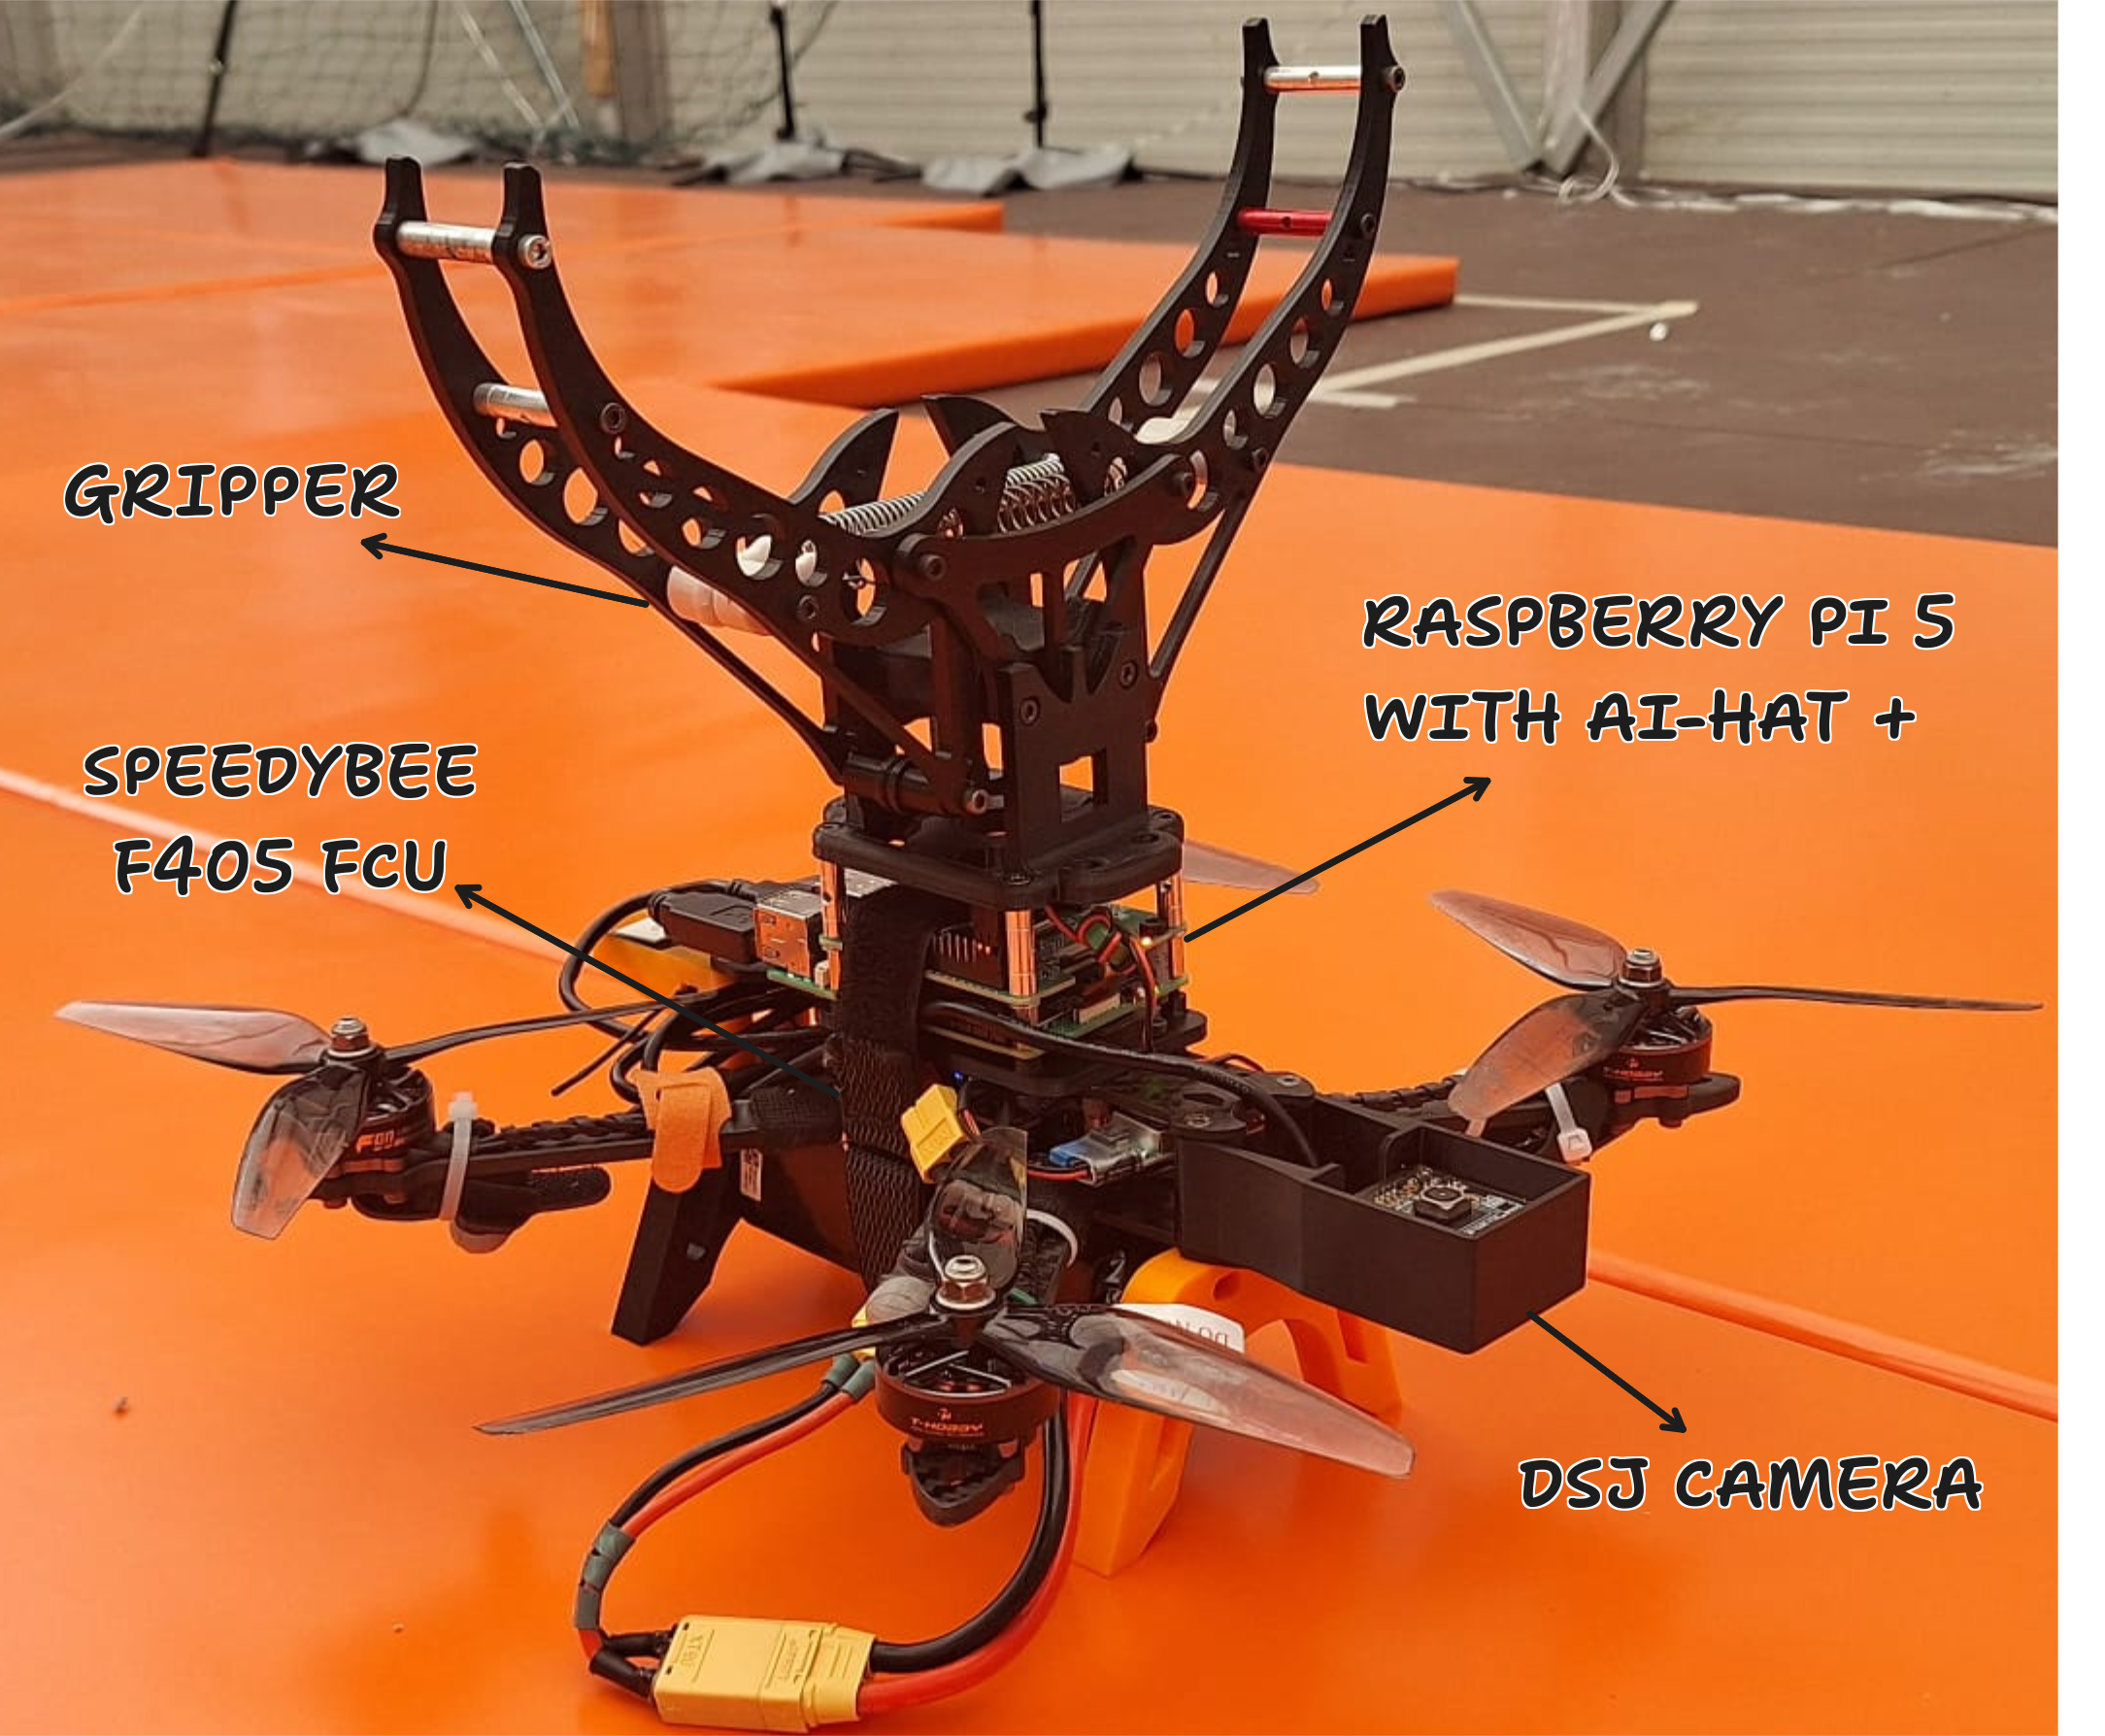
\includegraphics[width=0.85\textwidth]{images/uav_platform.png}
\caption{Letjelica korištena u eksperimentima s označenim glavnim komponentama: hvataljkom za prijanjanje, SpeedyBee F405 upravljačkom jedinicom, Raspberry Pi 5 računalom s AI Hat+ dodatkom te DSJ kamerom.}
\label{fig:uav_platform}
\end{figure}

\subsection{Računalo i senzori na letjelici}
Računalo na letjelici je Raspberry Pi 5 s 8 GB radne memorije, uz Raspberry Pi AI Hat+ dodatak s Hailo-8 akceleratorom (28 TOPS) za sklopovski ubrzano zaključivanje modela. Kao izvor slike koristi se DSJ-3079-HE, standardna USB (UVC) kamera spojena preko V4L2/OpenCV sučelja bez potrebe za posebnim upravljačkim programom, snima pri rezoluciji 1280×720 piksela i 30 sličica u sekundi.

\subsection{Mehanizam za prijanjanje}
Za prijanjanje se koristi prilagođena 3D-tiskana pasivna hvataljka s oprugom, izrađena od PETG materijala, montirana na okvir letjelice. Hvataljka ostaje otvorena dok se na unutarnji dio čeljusti ne primijeni dovoljna sila, nakon čega se hvataljka zatvara.

\section{Arhitektura sustava}
\label{sec:arhitektura}

% TODO: umetnuti dijagram arhitekture sustava

Sustav je podijeljen na dva izvedbena okruženja koja se izvode na istom fizičkom računalu (Raspberry Pi 5), ali u odvojenim programskim okolinama: Raspberry Pi OS, na kojem se izvodi percepcijski cjevovod, i Ubuntu unutar Docker kontejnera, na kojem se izvodi ROS upravljački sloj. Ta se podjela zadržava jer AI Hat+ akcelerator komunicira isključivo s Raspberry Pi OS okruženjem, pa sve što ovisi o slikovnim podacima i modelima dubokog učenja ostaje na toj strani.

Percepcijski cjevovod (poglavlje~\ref{ch:percepcija}) na ulazu preuzima okvire s kamere, a na izlazu proizvodi jednu pikselnu točku prijanjanja u slikovnoj ravnini. Ta se točka šalje preko UDP-a u Docker okruženje, gdje je preuzima upravljački sloj (poglavlje~\ref{ch:upravljanje}) koji je preslikava u naredbe kutne brzine tijela i brzine penjanja za letjelicu. Sučelje između dviju strana sustava jest jednostavna poruka koja nosi pikselnu poziciju ciljne točke u slici (\texttt{point\_x}, \texttt{point\_y}), čime se zadržava jasna granica između percepcije (koja ne zna ništa o geometriji letjelice ni o načinu upravljanja) i upravljanja (koje ne zna ništa o tome kako je točka detektirana ni kojim je modelom dobivena).

Izbor UDP-a kao poveznice između dviju strana sustava posljedica je same podjele na odvojena izvedbena okruženja: Raspberry Pi OS i Docker kontejner ne dijele isti procesni prostor, pa izravno dijeljenje memorije ili poziv funkcija nije moguć, a jedina veza između njih jest mrežno sučelje. Budući da se prenosi samo jedna točka po sličici, bez potrebe za jamstvom isporuke ili redoslijeda, UDP je dovoljan i jednostavniji od uspostave punog ROS mosta ili TCP veze između okruženja.

Percepcijska i upravljačka strana sustava rade na različitim, međusobno neusklađenim taktovima. Izlazna frekvencija modela detekcije nije fiksna: ovisi o vrsti detekcije i broju grana prisutnih u kadru, a kod stvarne detekcije grana na Raspberry Pi 5 pada na oko 4,6 Hz unatoč tome što kamera isporučuje 30 sličica u sekundi (vidi Odjeljak~\ref{sec:treniranje-modela}). Upravljački sloj \texttt{ibvs\_perching} naredbe objavljuje znatno češće, pri 30 Hz, pa bi izravno oslanjanje na izlaz modela detekcije u svakoj iteraciji upravljačke petlje predstavljalo usko grlo. Taj se problem rješava KLT praćenjem: nakon zaključavanja točke prijanjanja, model detekcije prestaje raditi, a značajke izdvojene iz referentne slike prate se optičkim tokom znatno većom frekvencijom, čime upravljački sloj u svakoj iteraciji prima ažuriranu procjenu položaja cilja, a ne zastarjelu vrijednost iz posljednjeg pokretanja modela. Detaljan opis ovog mehanizma dan je u Odjeljku~\ref{subsec:klt}.

Ovakva podjela odgovornosti nije samo posljedica sklopovskog ograničenja (Hailo-8 akcelerator dostupan isključivo na strani Raspberry Pi OS-a), nego i namjeran dizajnerski izbor koji dopušta zamjenu percepcijske strane bez izmjene upravljačkog sloja. To je u ovom radu i iskorišteno: isti upravljački sloj korišten je i s ArUco modulom za detekciju oznaka (poglavlje~\ref{ch:eksperimenti}) i s cjevovodom za detekciju grane, budući da oba proizvode identično sučelje prema Docker strani.


\chapter{Percepcija i praćenje točke prijanjanja}
\label{ch:percepcija}
\section{Pregled cjevovoda za detekciju}
\label{sec:pregled-cjevovoda}

Cjevovod za detekciju grane obrađuje isključivo slikovnu ravninu i ne sadrži ugrađenu pretpostavku o fizičkoj orijentaciji kamere u prostoru. Cjevovod za detekciju grane nije zaseban proces koji radi usporedno s praćenjem, nego je ugniježđen unutar iste petlje: dok konačna točka nije zaključana, svaka iteracija ove petlje poziva cjevovod za detekciju za sljedeću sličicu i iz njega čita trenutno stanje. Tek nakon zaključavanja petlja prestaje pozivati cjevovod za detekciju i prelazi na izravno čitanje sirovih sličica s kamere, a praćenje preuzima KLT algoritam opisan u nastavku (Odjeljak~\ref{subsec:klt}). Izlaz cjevovoda prema upravljačkom sloju ostaje par vrijednosti procijenjenog položaja točke prijanjanja u slikovnoj ravnini (\texttt{point\_x}, \texttt{point\_y}).

\section{Skup podataka i treniranje modela}
\label{sec:treniranje-modela}

Detekcija grana za primjene na UAV-u dosad je istraživana u nekoliko smjerova. Silva i sur.~\cite{SILVA2022102759} predložili su metodu detekcije linija temeljenu na konvolucijskoj neuronskoj mreži za prepoznavanje grana stabla iz digitalnih fotografija, koristeći Houghovu transformaciju za procjenu orijentacije grane i točke prihvata. Lin i sur.~\cite{lin2025performanceevaluationdeeplearning} usporedili su nekoliko modela dubokog učenja za segmentaciju u autonomnim šumarskim sustavima, dajući usporedbu performansi modela u stvarnim uvjetima. Oba rada usredotočena su isključivo na percepcijsku stranu problema, bez obrade cjelokupnog cjevovoda od detekcije do upravljanja, za razliku od njih, model korišten u ovom radu dio je cjelovitog cjevovoda opisanog u nastavku ovog poglavlja.

\subsection{Skup podataka i označavanje}
Izbor modela za segmentaciju instanci umjesto obične detekcije izravna je posljedica zahtjeva za pikselnom preciznošću točke prijanjanja. Okvir za detekciju (\emph{bounding box}) daje samo grubu procjenu položaja i veličine grane, dok manevar prijanjanja zahtijeva mnogo precizniju procjenu: pogreška od svega nekoliko centimetara u stvarnom prostoru dovoljna je da hvataljka fizički promaši granu. Maska na razini piksela, za razliku od okvira, omogućuje izdvajanje znatno preciznije točke unutar same grane, što je motivacija za korištenje segmentacijskog, a ne isključivo detekcijskog modela.

Skup podataka za treniranje preuzet je s Roboflowa~\cite{branch-dataset_dataset} i sadrži 1365 slika za treniranje, 390 za validaciju i 203 za testiranje, sve iz jedne klase (grana), izvorno označene okvirima za detekciju objekata. Budući da je za ovaj rad potrebna preciznost na razini piksela, a ne samo okvir, maske za segmentaciju automatski su generirane modelom SAM3 (Segment Anything Model 3) tvrtke Meta~\cite{carion2026sam3segmentconcepts}, na temelju tekstualnog upita "tree branch", čime se izbjeglo ručno označavanje gotovo 2000 slika. Puna segmentacija cijele scene izravnim pokretanjem SAM3 na ulazne okvire razmatrana je, ali odbačena kao računalno prezahtjevna za izvođenje na Raspberry Pi računalu.

\subsection{Treniranje i usporedba modela}
Treniranje je provedeno korištenjem Ultralytics biblioteke, koja objedinjuje sučelje za treniranje, validaciju i izvoz YOLO modela. Segmentacijski model YOLOv8m-seg treniran je 300 epoha, uz praćenje napretka na platformi Weights \& Biases. Usporedba je provedena i s modelom YOLOv26-seg treniranim pod istim uvjetima: YOLOv8m-seg dosljedno je nadmašio YOLOv26-seg po gotovo svim mjerama (npr. mAP50-95 na razini okvira približno 0,63 naspram 0,58), a uz to je i jedina opcija podržana za izvoz u format koji AI Hat+ prihvaća, budući da akcelerator podržava samo YOLO modele do verzije 8. YOLOv8m-seg stoga je odabran po oba kriterija.

Gubitci na skupu za treniranje i validaciju padaju i konvergiraju kroz svih 300 epoha, što ukazuje da model ne prenaučava (\emph{overfitting}) na skup za treniranje. Većina učenja odvija se unutar prvih 150 epoha, nakon čega mjere počinju stagnirati. mAP50 na razini okvira dosegnuo je približno 0,75 do kraja treniranja, što je razuman rezultat s obzirom na težinu zadatka: razlikovanje tanke, granate grane od pozadine sličnog izgleda (druge grane, sjene, tekstura kore) u prirodnom okruženju.

\begin{figure}[htb]
\centering
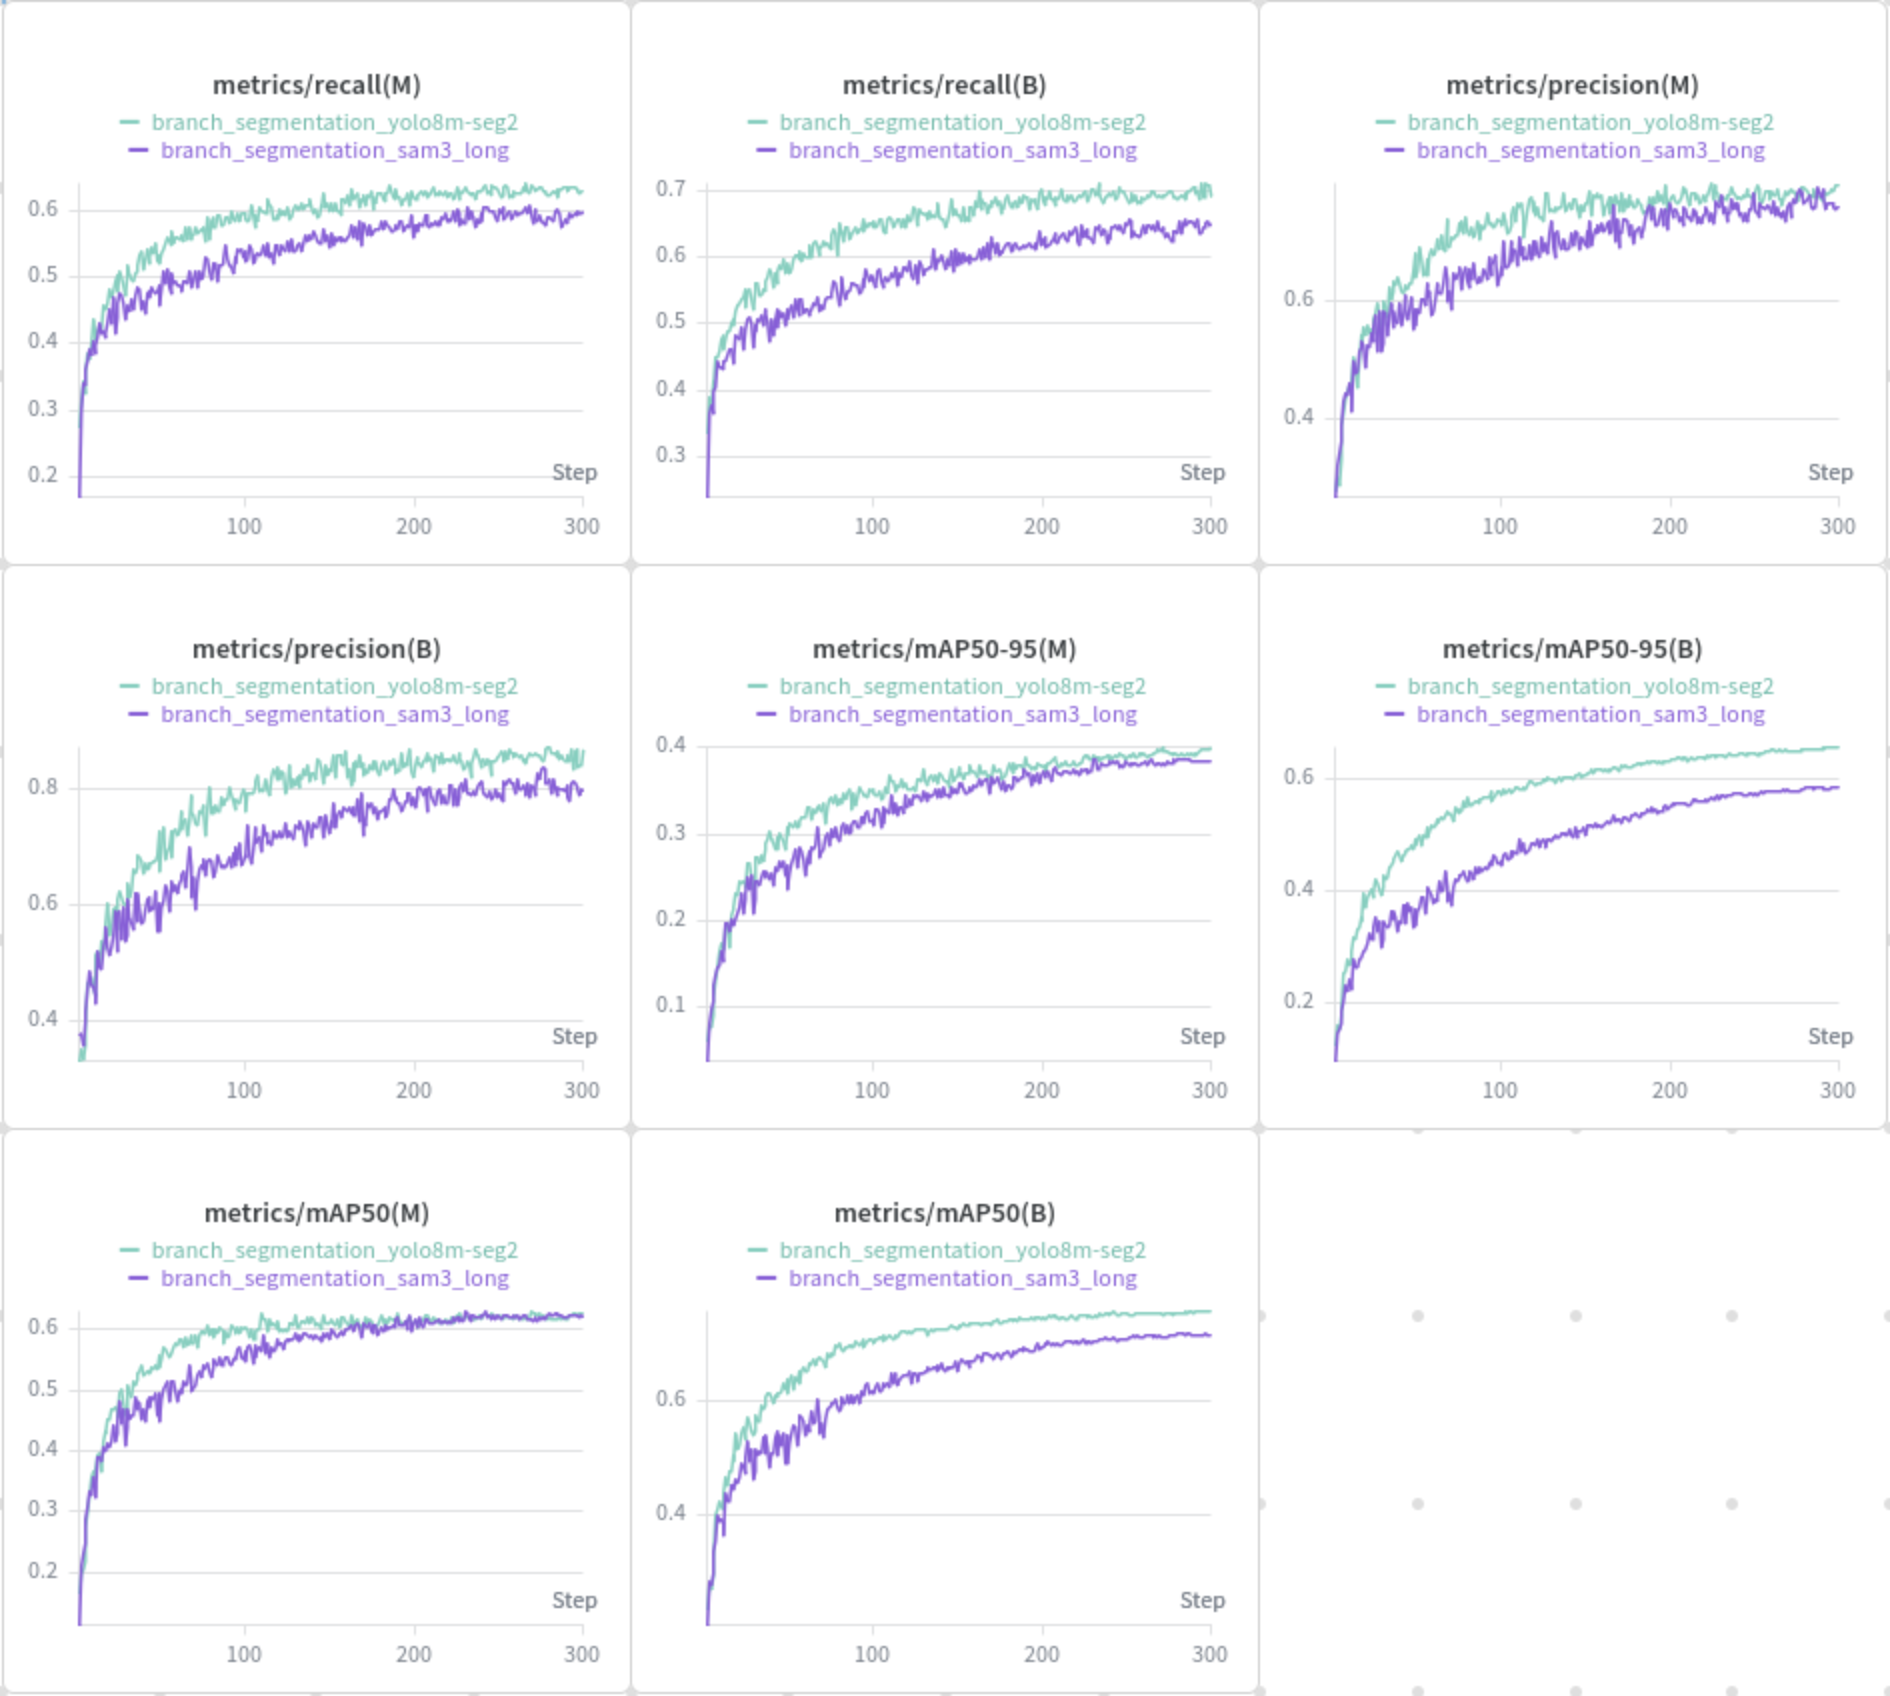
\includegraphics[width=1.0\textwidth]{images/metrics_compare.png}
\caption{Usporedba mjera treniranja modela YOLOv8m-seg i YOLOv26-seg kroz 300 epoha (odziv, preciznost i mAP na razini maske (M) i okvira (B)).}
\label{fig:metrics_compare}
\end{figure}

\subsection{Kvantizacija i izvođenje na rubnom uređaju}
\label{subsec:kvantizacija}
Nakon treniranja, težine modela izvezene su iz PyTorch (\texttt{.pt}) formata u ONNX, standardizirani format koji omogućuje prijenos modela između različitih okvira i sklopovlja. ONNX model potom je kompiliran u Hailo izvršni format (\texttt{.hef}) korištenjem Hailo AI Software Suite alata, koji Hailo distribuira kao Docker sliku sa svim potrebnim alatima. Nakon kvantizacije, brzina izvođenja modela na AI Hat+ akceleratoru ovisi o vrsti detekcije i broju grana prisutnih u kadru: unatoč tome što kamera isporučuje 30 sličica u sekundi, obrada na Raspberry Pi 5 pri stvarnoj detekciji grana usporava izlaznu frekvenciju cjevovoda na oko 4,6 Hz. Ovo usko grlo izravan je razlog uvođenja KLT praćenja nakon zaključavanja točke prijanjanja (vidi Odjeljak~\ref{subsec:klt}), koje zaobilazi ponovljeno pokretanje modela detekcije za svaku sličicu.

% TODO: napomenuti u Raspravi da skup podataka trenutno ne sadrzi fotografije grana
% snimljene iz perspektive kamere okrenute prema gore (nebo kao pozadina), sto moze
% utjecati na tocnost detekcije u novoj konfiguraciji

\section{Praćenje točke prijanjanja (KLT)}
\label{subsec:klt}

\begin{figure}[htb]
\centering
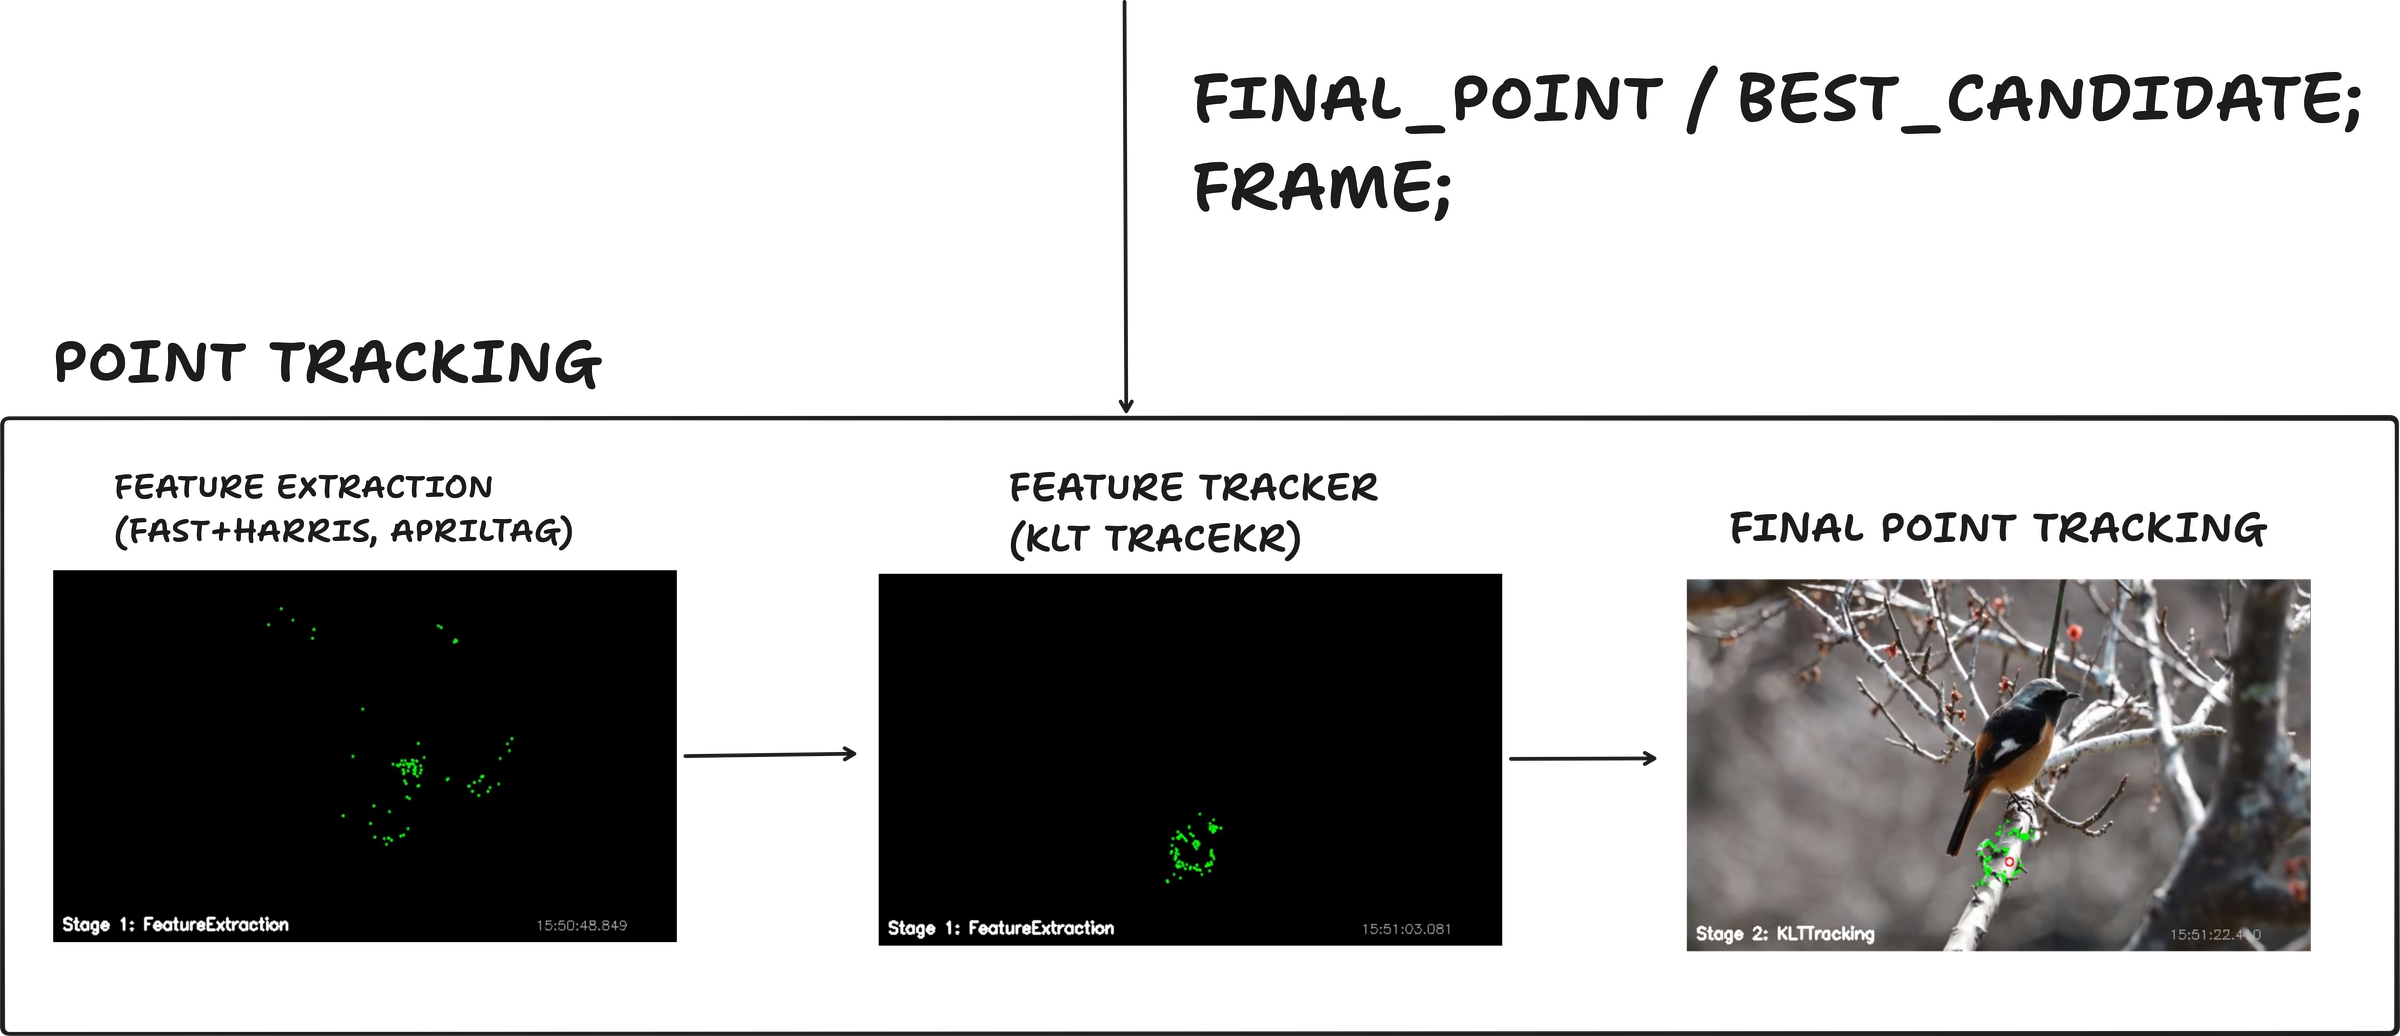
\includegraphics[width=1.0\textwidth]{images/point_tracking_overview.png}
\caption{Integracija cjevovoda za detekciju s praćenjem točke prijanjanja: izdvajanje značajki, KLT praćenje i procjena položaja konačne točke.}
\label{fig:ibvs_overview}
\end{figure}

Nastavak oslanjanja na model segmentacije nakon zaključavanja točke bio bi neopravdano skup: kako je pokazano u Odjeljku~\ref{subsec:kvantizacija}, izlazna frekvencija modela detekcije pri stvarnoj detekciji grana pada na oko 4,6 Hz, dok upravljački sloj zahtijeva znatno češće ažuriranje cilja. Umjesto ponovnog pokretanja modela, praćenje se stoga oslanja isključivo na optički tok, koji je računalno jeftiniji i ne ovisi o ponovljenom uspješnom prepoznavanju grane u svakoj sličici. Ovo praćenje izvodi se u potpunosti na strani Raspberry Pi OS-a, kao dio istog procesa koji izvodi cjevovod za detekciju, za razliku od upravljačke IBVS petlje opisane u poglavlju~\ref{ch:upravljanje}, koja se izvodi zasebno, na Docker strani sustava.

Nakon zaključavanja konačne točke, KLT tracker izdvaja FAST i Harris kutne značajke iz referentne slike u lokalnoj okolini točke prijanjanja te pohranjuje pomak svake značajke u odnosu na tu točku.

U svakoj sljedećoj slici značajke se prate KLT (\emph{Kanade--Lucas--Tomasi}) algoritmom optičkog toka na piramidalnoj reprezentaciji slike, a položaj točke prijanjanja procjenjuje se kao trenutno središte (centroid) uspješno praćenih značajki. Time se izbjegava ponovno pokretanje modela detekcije za svaku sliku, čime se smanjuje računalno opterećenje i omogućuje praćenje znatno većom frekvencijom nego što bi to dopuštalo izvođenje modela segmentacije nad svakim okvirom.

\begin{figure}[htb]
\centering
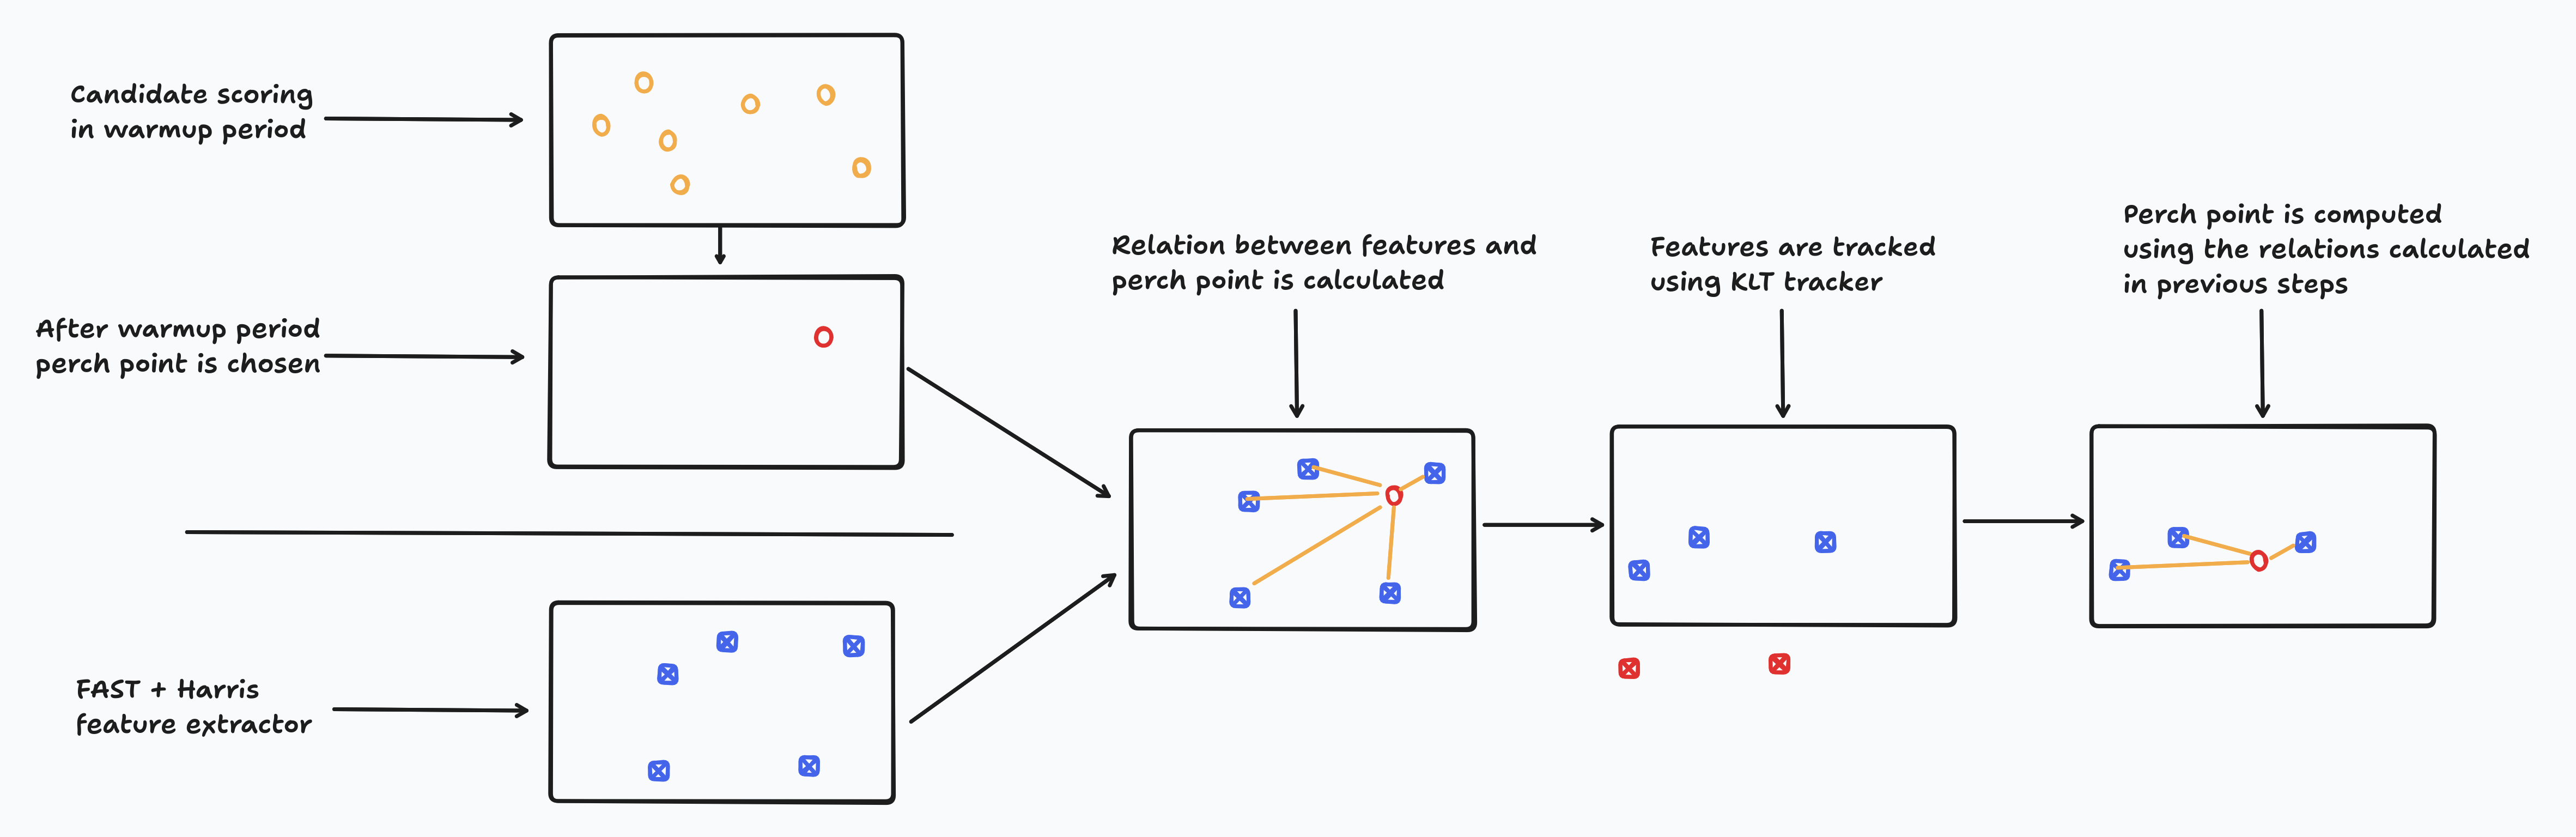
\includegraphics[width=1.0\textwidth]{images/final_point_tracking.png}
\caption{Postupak procjene položaja točke prijanjanja: odnos između izdvojenih značajki i zaključane točke fiksira se u trenutku zaključavanja, a nakon svakog koraka KLT praćenja taj se fiksni odnos primjenjuje na nove položaje značajki kako bi se odredio procijenjeni položaj točke. Testni video~\cite{pixabay_bird_video}.}
\label{fig:final_point_tracking}
\end{figure}

Praćenje uključuje provjeru dosljednosti unaprijed-unatrag (\emph{forward-backward}): svaka procijenjena nova pozicija značajke prati se i unatrag u prethodnu sliku, a značajke čiji povratni položaj odstupa od izvornog odbacuju se kao nepouzdane. Ako broj preživjelih značajki padne ispod praga, značajke se ponovno izdvajaju oko predviđenog položaja središta (na temelju posljednje zabilježene brzine pomaka), umjesto oko posljednjeg poznatog položaja, čime se ponovno izdvajanje bolje prilagođava kretanju cilja. Dodatno, ako se središte praćenih značajki ne pomiče kroz veći broj uzastopnih slika, praćenje se proglašava nepouzdanim i signalizira se gubitak cilja, čime se sprječava da sustav neprimjetno prati nepomičnu pozadinu umjesto stvarnog cilja.

Pogreška u odnosu na središte slike ovdje se ne računa: taj izračun, kao i preslikavanje u naredbe letjelici, u potpunosti je izmješten u upravljačku IBVS petlju opisanu u poglavlju~\ref{ch:upravljanje}, koja se izvodi zasebno, na Docker strani.


\chapter{Upravljanje letjelicom}
\label{ch:upravljanje}
\section{Sučelje prema percepciji}
\label{sec:sucelje-percepcija}

\subsection{Prijenos podataka između percepcije i upravljanja}
\label{subsec:udp-most}

Budući da se percepcijski cjevovod i upravljački sloj izvode u odvojenim izvedbenim okruženjima na istom računalu (poglavlje~\ref{ch:sustav}), potreban je most između njih. Percepcijska strana šalje UDP paket u JSON formatu, koji sadrži dvije vrijednosti (\texttt{px}, \texttt{py}), pikselnu poziciju ciljne točke zaokruženu na cijeli broj. Slanje obavlja jednostavna UDP utičnica (\emph{socket}) klase \texttt{UDPSender}, koja paket šalje na unaprijed zadanu IP adresu i port (5005) Docker okruženja pri svakoj sličici za koju postoji ciljna točka, bez potvrde primitka ili ponovnog slanja u slučaju gubitka paketa.

Na Docker strani, namjenski ROS čvor prima paket, popunjava poruku tipa \texttt{PointStamped} vrijednostima \texttt{point.x} i \texttt{point.y}, dok se \texttt{point.z} uvijek postavlja na nulu budući da sustav ne raspolaže mjerenjem udaljenosti do cilja, te je objavljuje na temu \texttt{ibvs/target\_point}, izvorno sučelje koje paket \texttt{ibvs\_perching} inače koristi s vlastitim (ArUco) modulom percepcije. Time se omogućuje da isti upravljački sloj prima ciljnu točku i od ArUco modula i od cjevovoda za detekciju grane, bez izmjena u samom upravljanju. Naredba za vertikalno kretanje ne izvodi se iz ove poruke, nego je unaprijed zadana konstanta u upravljačkom sloju (vidi Odjeljak~\ref{subsec:prijanjanje}).

\subsection{Preslikavanje osi za kameru okrenutu prema gore}
\label{subsec:preslikavanje-osi}

% TODO: ovo poglavlje dovrsiti nakon eksperimentalne provjere stvarnog predznaka i
% osi -- trenutno opisuje namjeravano ponasanje, ne izmjereno

Paket \texttt{ibvs\_perching} izvorno pretpostavlja kameru okrenutu prema dolje, gdje vodoravni pomak u slici odgovara pomaku unaprijed, a okomiti pomak pomaku ulijevo/udesno. U ovom radu, s kamerom okrenutom prema gore, vodoravni pomak u slici umjesto toga upravlja bočnim nagibom, a okomiti pomak nagibom naprijed-natrag, dok os prilaska (penjanje) preuzima ulogu koju je izvorno imao pomak unaprijed. Upravljački sloj ne koristi nikakav vanjski koordinatni sustav, nego se oslanja isključivo na vlastitu inercijsku/AHRS procjenu orijentacije letjelice, pa je preslikavanje osi jedina prilagodba potrebna za rad s kamerom okrenutom prema gore. Obje se osi pritom normaliziraju istom polovinom širine slike, a ne svaka svojom polovinom dimenzije, budući da bi dijeljenje okomite pogreške njezinom vlastitom, manjom polovinom visine slike isto pojačanje regulatora učinilo jačim na toj osi.

\section{Upravljačka petlja}
\label{sec:upravljacka-petlja}

Na strani upravljanja, Ji i sur.~\cite{ji2022realtimetrajectoryplanningaerial} predstavili su metodu planiranja trajektorije u stvarnom vremenu za zračno prijanjanje. Samadikhoshkho i Lipsett~\cite{drones8110605} kombinirali su duboko učenje s vizualnim navođenjem temeljenim na slici za zračno uzorkovanje vegetacije. Domišlović i sur.~\cite{domislovic_marsupial} demonstrirali su vizualno navođenje temeljeno na poziciji s marsupijalnim robotskim sustavom, pristup srodan onome korištenom u ovom radu. Kim i Chang~\cite{drones10040270} predstavili su sustav prijanjanja bez markera za kvadrokopter koji kombinira model segmentacije sa senzorom udaljenosti i upravljačem temeljenim na konačnom automatu, izvodeći cijeli cjevovod na Jetson Orin NX platformi. Do i Hong~\cite{do2023visionbased} ostvarili su vizualno prijanjanje nano letjelice na vodoravnu površinu korištenjem monokularne kamere i procjene poze u odnosu na oznaku. He i sur.~\cite{he2023imagebased} primijenili su vizualno navođenje temeljeno na slici za zračnu manipulaciju potpuno pokretljivom letjelicom, prateći linijske značajke umjesto točkastih. Mao i sur.~\cite{mao2023robust} razvili su robusno aktivno vizualno prijanjanje kvadrokoptera na nagnute površine uz ponovno planiranje putanje u stvarnom vremenu. Di i sur.~\cite{di2026slap} predstavili su sustav prijanjanja na okomita debla drveća koji kombinira vizualnu detekciju mjesta prijanjanja s IMU-temeljenom detekcijom neuspjelog pokušaja i mehanizmom oporavka. Za razliku od ovih pristupa, koji redom pretpostavljaju raspoloživ sustav apsolutne lokalizacije, senzor udaljenosti za okidanje prijanjanja ili poznatu oznaku/površinu cilja, upravljački sloj korišten u ovom radu ne oslanja se ni na jedno od toga.

Letjelicom upravlja paket \texttt{ibvs\_perching}~\cite{ibvs_perching}, izgrađen nad ArduPilot autopilotom i MAVROS mostom prema ROS-u~\cite{aliane2024survey}. Taj paket ne koristi kontroler pozicije niti vanjsku lokalizaciju: letjelicom upravlja izravno preko sučelja \texttt{mavros/setpoint\_raw/attitude}, šaljući ciljnu orijentaciju letjelice za bočno poravnanje (Odjeljak~\ref{subsec:pid-kaskada}) te naredbu brzine penjanja (kroz polje \texttt{thrust}, protumačeno u ArduPilot GUIDED načinu rada kao naredba brzine penjanja, a ne kao sirovi potisak) za okomiti prilazak.

\subsection{Kaskadni regulator položaja}
\label{subsec:pid-kaskada}

Vodoravno poravnanje ostvaruje se kaskadnom strukturom s dvije razine. Vanjska petlja preslikava normaliziranu pikselnu pogrešku u željeni nagib letjelice (\emph{tilt}) preko dva neovisna PID regulatora, jednog za svaku os. Pojačanje regulatora izraženo je u radijanima nagiba po jediničnoj pogrešci, tako da izlaz regulatora izravno predstavlja nagib koji se naređuje na rubu slike, a ne kutnu brzinu. Integralni član sprječava trajno odstupanje u prisutnosti stalnog poremećaja poput vjetra, dok derivacijski član, izračunat iz razlike uzastopnih detekcija, unaprijed koči prilazak i ublažava nadmašaj. Derivacijski član zanemaruje se ako je razmak između dvije uzastopne detekcije predugačak, budući da bi u tom slučaju izražavao stvarno pomicanje cilja, a ne brzinu njegova kretanja u odnosu na letjelicu.

\begin{figure}[htb]
\centering
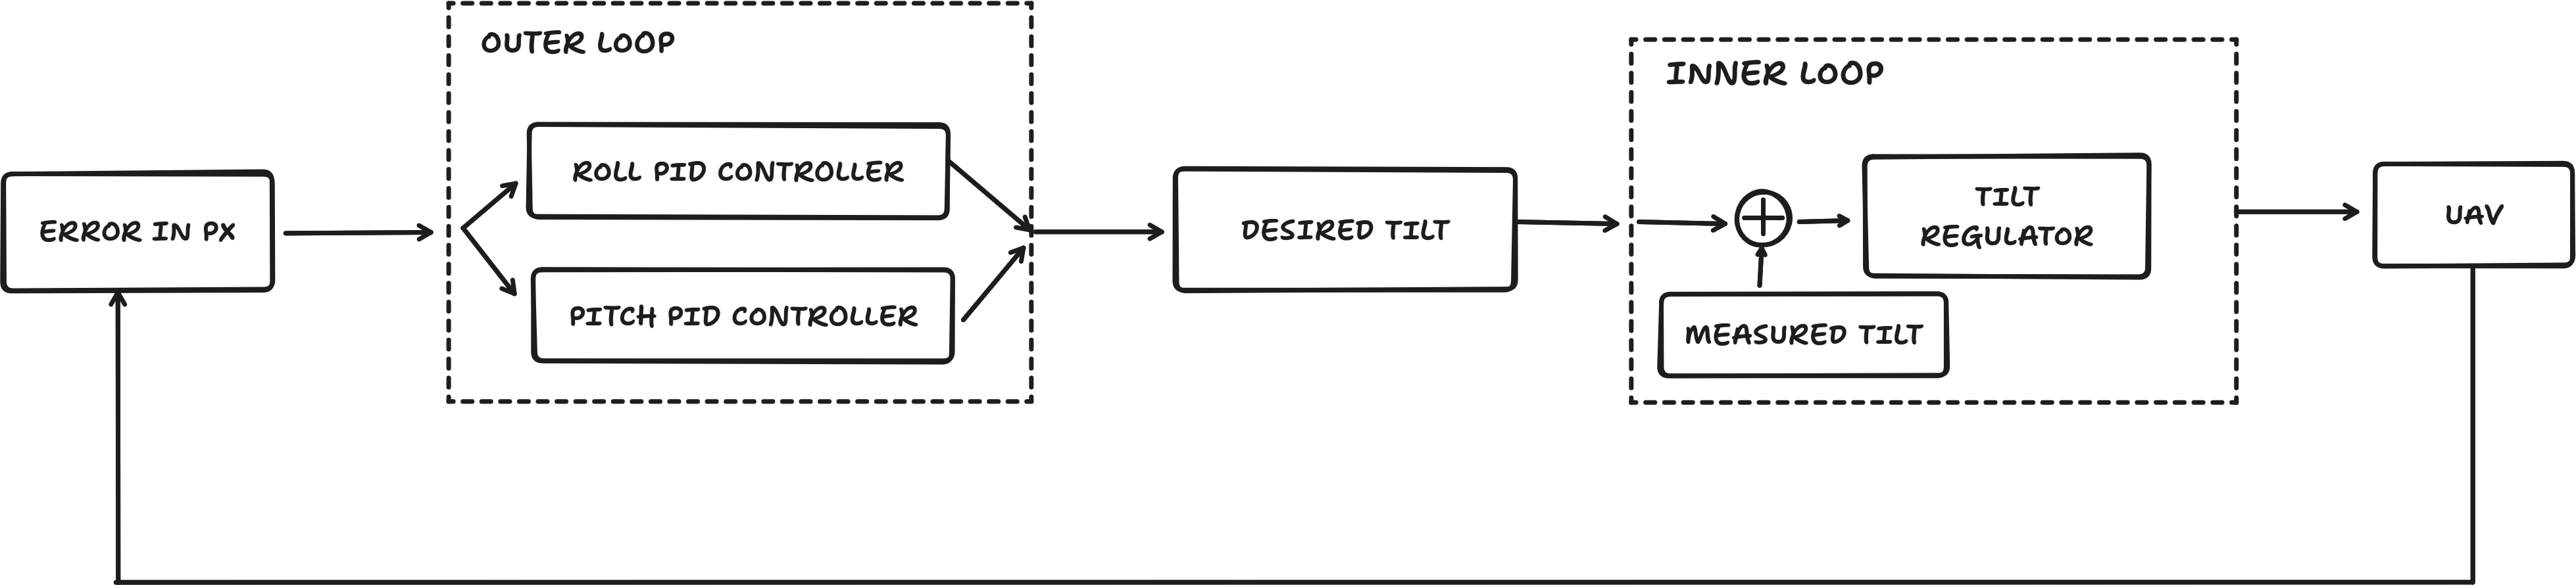
\includegraphics[width=1.0\textwidth]{images/cascade_controller.png}
\caption{Kaskadni regulator položaja: vanjska petlja (dva PID regulatora, po jedan za svaku os) preslikava pikselnu pogrešku u željeni nagib, koji se u \emph{attitude} načinu šalje kao ciljna orijentacija unutarnjoj petlji ArduPilota.}
\label{fig:cascade_controller}
\end{figure}

Izlaz vanjske petlje, željeni nagib, letjelici se predaje na jedan od dva načina, odabran postavkom upravljačkog sloja. U uobičajenom načinu (\emph{attitude}) željeni nagib šalje se izravno kao ciljna orijentacija (kvaternion), a unutarnju petlju koja tu orijentaciju pretvara u stvarnu kutnu brzinu zatvara sam ArduPilot, koristeći vlastite, tvornički ugođene regulacijske parametre pri visokoj frekvenciji. Alternativni način (\emph{rate}) šalje izravno naredbu kutne brzine tijela, izračunatu jednostavnim proporcionalnim regulatorom iz razlike između željenog i trenutnog nagiba, gdje se trenutni nagib očitava iz AHRS procjene orijentacije letjelice (poglavlje~\ref{sec:teorijska-podloga}). Ovaj se način koristi isključivo za usporedbu na klupi, dok se u letu koristi prvi način.

Izbor načina \emph{attitude} za let nije proizvoljan: raniji pokušaji leta u načinu \emph{rate} pokazali su da naredba nagiba u smjeru propinjanja (\emph{pitch}) zasićuje na graničnoj vrijednosti (\texttt{max\_tilt}) u velikoj većini uzoraka tijekom poravnanja, budući da jednostavan proporcionalni regulator kutne brzine, bez unutarnje petlje koju bi zatvarao autopilot, sporije i nestabilnije prati zadani nagib. Prelaskom na \emph{attitude} način, ArduPilotova vlastita, tvornički ugođena unutarnja petlja preuzima to zatvaranje pri znatno višoj frekvenciji, čime se zasićenje izbjeglo i let postao stabilniji. Neovisno o odabranom načinu, kruta veza između kamere i tijela letjelice unosi i fizičku vezanost između naređenog nagiba i same slike: svaki nagib koji regulator naredi istovremeno zakreće vidokrug kamere, što se u pikselnoj pogreški očituje kao kratkotrajan skok neposredno prije nego što stvarno translacijsko gibanje letjelice počne pogrešku smanjivati. Ova je vezanost svojstvena samoj geometriji sustava, a ne posljedica odabira načina slanja naredbe, i razmatra se i u poglavlju~\ref{ch:rezultati} na stvarnim podacima leta.

Naredba nagiba ograničena je unaprijed zadanom maksimalnom vrijednošću, neovisno o veličini pikselne pogreške. Ovo ograničenje ujedno predstavlja i glavnu sigurnosnu granicu sustava: bez obzira na to koliko velika pogreška u slikovnoj ravnini bude, ili kako pogrešno predznak preslikavanja osi bude postavljen, letjelica se ne može nagnuti strmije od ove granice, čime se ograničava i najveća moguća brzina vodoravnog pomicanja.

\subsection{Stanje sustava}
\label{subsec:state-machine}

Upravljački sloj strukturiran je kao konačni automat sa sedam stanja, koji određuje smije li se u danom trenutku uopće izvoditi poravnanje ili vertikalno kretanje. Letjelica polazi u stanju čekanja naoružavanja, u kojem se naredbe nagiba i penjanja drže na neutralnim vrijednostima (razina i lebdenje). Nakon što je letjelica naoružana i prebačena u odgovarajući način leta, sustav prelazi u stanje mirovanja ako cilj trenutno nije vidljiv, odnosno u stanje pripravnosti ako je cilj u tom trenutku vidljiv (potonje je isključivo informativna oznaka operateru da je poravnanje spremno početi). Servoiranje se aktivira zasebnim zahtjevom (uslugom), nakon čega sustav prelazi u stanje poravnanja te, kada pogreška padne ispod praga i ondje ostane dovoljno dugo, u stanje poravnano, u kojem se izvodi i vertikalno kretanje opisano u nastavku. Ako se cilj tijekom poravnanja ili nakon njega izgubi na razdoblje dulje od unaprijed određenog praga, sustav prelazi u stanje izgubljenog cilja, u kojem se letjelica vraća na razinu i miruje dok se cilj ponovno ne pojavi.

Izlazak iz stanja poravnano zahtijeva da pogreška premaši prag pomnožen histereznim faktorom, čime se sprječava treperenje između stanja poravnanja i poravnano oko same granice praga. Iz bilo kojeg stanja, gubitak naoružanja ili napuštanje odgovarajućeg načina leta letjelicu odmah vraća u stanje čekanja naoružavanja, neovisno o tome što se u tom trenutku događalo. Ova zaštita djeluje neovisno o softveru upravljačkog sloja: promjena načina leta obavlja se isključivo ručno, preko prekidača na daljinskom upravljaču sigurnosnog pilota, pa upravljački sloj nikada sam ne preuzima niti prepušta kontrolu nad letjelicom. Time sigurnosni pilot u svakom trenutku zadržava mogućnost trenutačnog preuzimanja ručnog upravljanja, neovisno o tome u kojem se stanju automat nalazi.

Sedam stanja u kodu nose nazive \texttt{WAIT\_ARM} (čekanje naoružavanja), \texttt{CLIMB} (penjanje pri uzlijetanju), \texttt{HOVER} (mirovanje), \texttt{TAG\_IN\_SIGHT} (pripravnost, cilj vidljiv), \texttt{ALIGN} (poravnanje), \texttt{ALIGNED} (poravnano) i \texttt{TAG\_LOST} (cilj izgubljen). Iz \texttt{WAIT\_ARM}, letjelica nakon naoružavanja prelazi u \texttt{CLIMB} ako je zatražen automatski uzlet, ili izravno u \texttt{ALIGN}/\texttt{TAG\_LOST} ako je servoiranje već zatraženo dok je letjelica bila naoružana i u letu. Iz \texttt{CLIMB}, po dosezanju ciljne visine, sustav prelazi u \texttt{HOVER}/\texttt{TAG\_IN\_SIGHT} ako servoiranje još nije pokrenuto, odnosno izravno u \texttt{ALIGN} ili \texttt{TAG\_LOST} ako jest. Stanja \texttt{HOVER} i \texttt{TAG\_IN\_SIGHT} razlikuju se isključivo po vidljivosti cilja i ponašaju se identično, dok se iz oba, na zaseban zahtjev za početak servoiranja, prelazi u \texttt{ALIGN}. Unutar \texttt{ALIGN}/\texttt{ALIGNED}, gubitak cilja dulje od praga (\texttt{tag\_timeout}) vodi u \texttt{TAG\_LOST}, iz kojeg se sustav vraća u \texttt{ALIGN} čim je cilj ponovno vidljiv. Iz bilo kojeg stanja u letu, zaseban zahtjev za zaustavljanje servoiranja vraća sustav u \texttt{HOVER}.

\begin{figure}[htb]
\centering
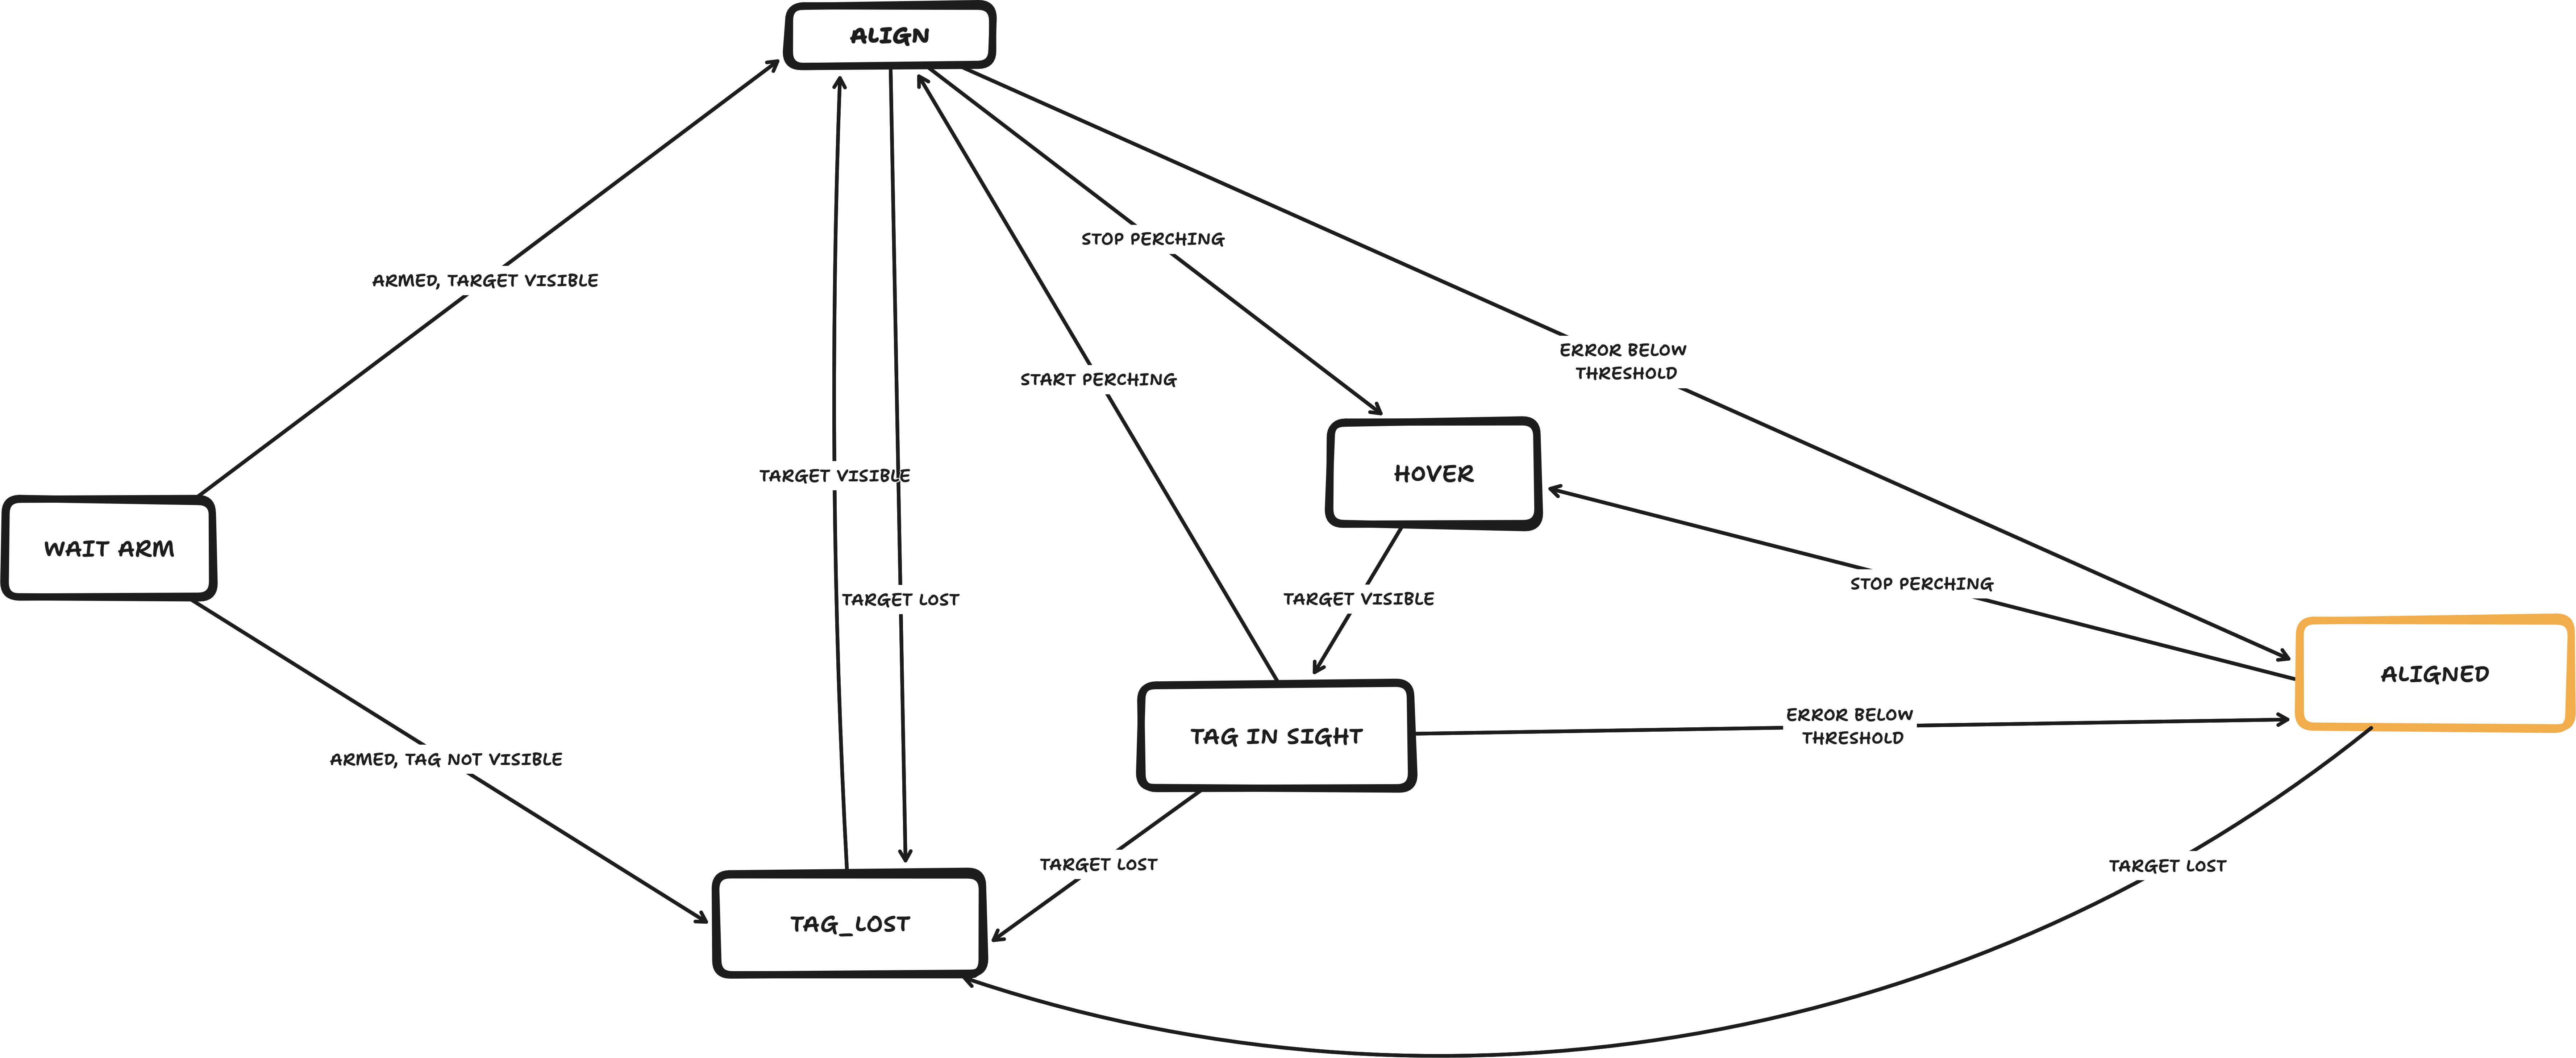
\includegraphics[width=1.0\textwidth]{images/state_machine.png}
\caption{Automat stanja upravljačkog sloja: sedam stanja i prijelazi između njih.}
\label{fig:state_machine}
\end{figure}

\subsection{Prilazak bez okidača temeljenog na mjerenju udaljenosti}
\label{subsec:prijanjanje}

Budući da senzor udaljenosti nije dostupan za okidanje manevra prijanjanja, vertikalno kretanje ne temelji se na izravnom mjerenju udaljenosti niti na bilo kojoj vrijednosti proslijeđenoj iz percepcijskog cjevovoda. Umjesto toga, upravljački sloj \texttt{ibvs\_perching} naredbu penjanja izvodi kao unaprijed zadanu konstantu (\texttt{perch\_climb\_thrust}), aktivnu u oba stanja poravnanja (poravnanje i poravnano, vidi Odjeljak~\ref{subsec:state-machine}) sve dok je bočna udaljenost detekcije od ciljne točke unutar zasebnog, šireg praga (\texttt{descend\_xy\_gate\_px}). Ta se udaljenost računa izravno iz sirove pikselne pogreške, neovisno o unutarnjoj normalizaciji regulacijske petlje, kako bi prag imao isto značenje bez obzira na to kako je regulator prethodno skalirao pogrešku. Time se izbjegava potreba za diskretnim okidačem temeljenim na mjerenju udaljenosti: penjanje se odvija kontinuirano dok je letjelica dovoljno bočno poravnata, umjesto da ga pokreće poseban signal iz percepcije ili zadržavanje u pojedinom stanju. Prag za penjanje namjerno je postavljen tako da nikad ne bude uži od praga koji definira ulazak u stanje poravnano, čime je osigurano da dosezanje stanja poravnano uvijek dopušta i penjanje. Penjanje ili spuštanje izvan tog praga izgurnulo bi granu iz vidnog polja kamere brže nego što bi je bočno poravnanje moglo ponovno uhvatiti.


\chapter{Eksperimenti}
\label{ch:eksperimenti}
Provjera sustava provedena je u tri koraka rastuće složenosti, gdje se u svakom sljedećem koraku mijenja točno jedna varijabla u odnosu na prethodni: prvo provjera upravljačkog sloja u njegovoj izvornoj konfiguraciji, zatim provjera prilagodbe za kameru okrenutu prema gore uz i dalje jednostavan i pouzdan cilj (ArUco oznaka), te naposljetku provjera cijelog sustava s cjevovodom za detekciju grane umjesto ArUco oznake. Ciljna točka u sva tri koraka do upravljačkog sloja stiže istim putem, UDP mostom opisanim u Odjeljku~\ref{subsec:udp-most}, tako da ta poveznica nije varijabla koja se mijenja između eksperimenata.

\section{Eksperiment 1: slijetanje na ArUco oznaku (kamera prema dolje)}
\label{sec:test1}

Cilj prvog eksperimenta jest provjeriti upravljački sloj (\texttt{ibvs\_perching}) u njegovoj izvornoj konfiguraciji, prije bilo kakve prilagodbe za scenarij prijanjanja na granu, te ugoditi odziv letjelice (parametre regulatora poravnanja) na ovoj jednostavnijoj konfiguraciji prije prelaska na složenije scenarije u drugom i trećem eksperimentu. Ciljnu točku i u ovom eksperimentu određuje isti cjevovod za detekciju opisan u poglavlju~\ref{ch:percepcija}, koji se koristi i u preostala dva eksperimenta, a ne modul za detekciju ArUco oznake ugrađen u paket \texttt{ibvs\_perching}. Razlika je u tome što cjevovod ovdje detektira ArUco oznaku umjesto grane, uz isključene filtre za ocjenjivanje kandidata koji su specifični za oblik i orijentaciju grane, dok ostatak cjevovoda, uključujući KLT praćenje i UDP most, ostaje nepromijenjen u sva tri eksperimenta.

\subsection{Postav}
\label{subsec:test1-postav}
ArUco oznaka postavljena je na tlo, a letjelica leti iznad nje s kamerom okrenutom prema dolje, izvorna konfiguracija paketa \texttt{ibvs\_perching}. Letjelica slijeće izravno na oznaku.

\section{Eksperiment 2: praćenje ArUco oznake (kamera prema gore)}
\label{sec:test2}

Cilj drugog eksperimenta jest izolirano provjeriti prilagodbu upravljačkog sloja za kameru okrenutu prema gore (Odjeljak~\ref{subsec:preslikavanje-osi}), zadržavajući ArUco oznaku kao jednostavan i pouzdan izvor ciljne točke. Time se promjena geometrije (kamera prema gore, cilj iznad letjelice) provjerava odvojeno od uvođenja cjevovoda za detekciju grane, koji je uveden tek u trećem eksperimentu. Budući da je kamera na letjelici radi ovog eksperimenta fizički zarotirana za 180 stupnjeva u odnosu na prvi eksperiment, cilj je ujedno i ispraviti preslikavanje osi tako da odgovara ovoj novoj orijentaciji kamere.

\subsection{Postav}
\label{subsec:test2-postav}
ArUco oznaka postavljena je na povišeno mjesto, a kamera na letjelici okrenuta je prema gore. Letjelica nastoji poravnati se s oznakom i prići joj odozdo.

\section{Eksperiment 3: prijanjanje na granu}
\label{sec:test3}

Cilj trećeg i glavnog eksperimenta jest provjeriti cijeli sustav opisan u ovom radu u konačnoj konfiguraciji: ArUco oznaka je uklonjena, a ciljnu točku određuje cjevovod za detekciju grane (poglavlje~\ref{ch:percepcija}), detekcija modelom, potom praćenje KLT algoritmom, čiji se izlaz UDP mostom prenosi upravljačkom sloju prilagođenom kameri okrenutoj prema gore (poglavlje~\ref{ch:upravljanje}).

\subsection{Postav}
\label{subsec:test3-postav}
Letjelica polazi pozicionirana neposredno ispod grane, s kamerom okrenutom prema gore. Potrebno je uzeti u obzir prostorni razmak između kamere i mehanizma za prijanjanje (hvataljke), budući da se ciljna točka određuje u odnosu na kameru, dok manevar prijanjanja mora dovesti granu u doseg hvataljke, a ne samo u središte slike.


\chapter{Rezultati i rasprava}
\label{ch:rezultati}
\section{Rezultati eksperimenata}
\label{sec:rezultati-eksperimenata}

Za sva tri eksperimenta opisana u poglavlju~\ref{ch:eksperimenti} prikazani su podaci snimljeni tijekom stvarnog leta (\emph{rosbag} zapis svih tema upravljačkog sloja), ograničeni na razdoblje u kojem je regulator poravnanja stvarno aktivan, od ulaska u stanje \texttt{ALIGN} do njegovog konačnog napuštanja. Svi kutovi na grafovima izraženi su u stupnjevima radi čitljivosti, iako ih upravljački sloj interno računa i objavljuje u radijanima.

\subsection{Eksperiment 1: slijetanje na ArUco oznaku (kamera prema dolje)}
\label{subsec:rez-eksperiment1}

Letjelica je iz stanja \texttt{ALIGN} krenula s pikselnom pogreškom od približno $(25, 40)$ piksela i regulator ju je unutar nešto manje od četiri sekunde sveo na vrijednost unutar praga poravnanja (Slika~\ref{fig:exp1-error}), nakon čega je sustav ušao u stanje \texttt{ALIGNED} i letjelica sletjela. Budući da je upravljački sloj u ovom letu radio u načinu \emph{attitude} (Odjeljak~\ref{subsec:pid-kaskada}), naredba se šalje kao ciljni nagib, a ne kutna brzina, pa je naređeni i stvarni nagib letjelice izravno usporediv na istom grafu. Oba usko prate jedan drugoga tijekom čitavog manevra (Slika~\ref{fig:exp1-angles}), uz zaostajanje AHRS procjene od otprilike 0.2 do 0.3 sekunde iza naredbe, posljedica dinamike letjelice i unutarnje petlje koju zatvara sam ArduPilot. Naredba okomitog kretanja (Slika~\ref{fig:exp1-thrust}) prelazi s vrijednosti mirovanja (0.5) na vrijednost spuštanja (\texttt{land\_descend\_thrust}, 0.45) čim je letjelica bočno unutar praga za spuštanje, i vraća se na mirovanje kad taj prag napusti, potvrđujući opisanu funkcionalnu ovisnost okomitog kretanja o bočnom poravnanju (Odjeljak~\ref{subsec:prijanjanje}).

\begin{figure}[h]
  \centering
  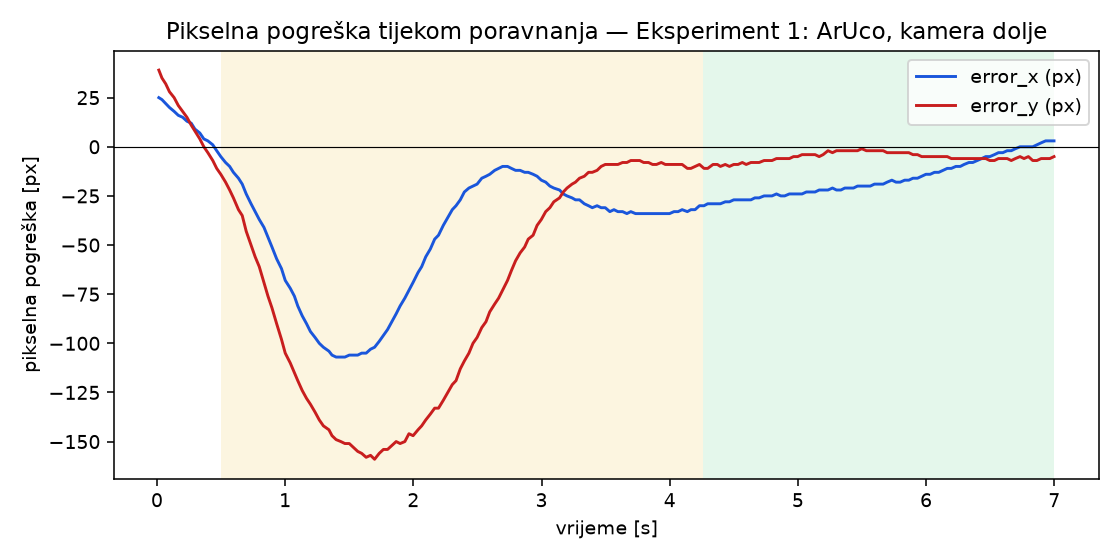
\includegraphics[width=0.85\textwidth]{images/rezultati/exp1_error.png}
  \caption{Pikselna pogreška tijekom prvog eksperimenta. Žuto osjenčano područje označava stanje \texttt{ALIGN}, zeleno stanje \texttt{ALIGNED}.}
  \label{fig:exp1-error}
\end{figure}

\begin{figure}[h]
  \centering
  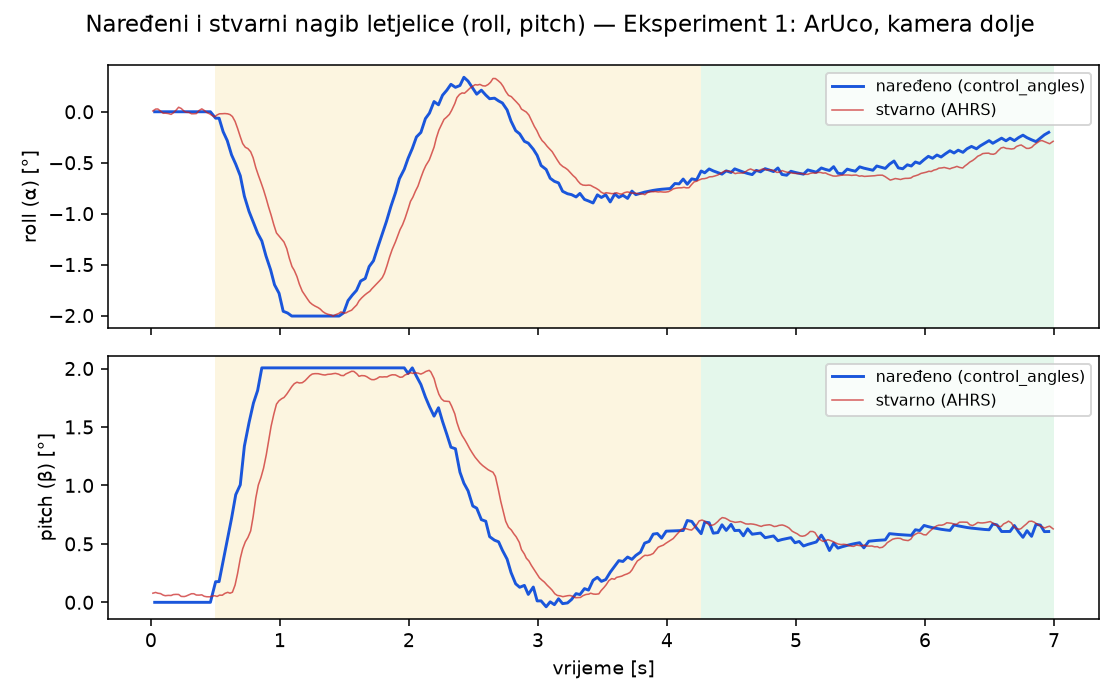
\includegraphics[width=0.85\textwidth]{images/rezultati/exp1_angles.png}
  \caption{Naređeni nagib (izlaz vanjske petlje, nakon ograničenja) i stvarni nagib očitan iz AHRS-a tijekom prvog eksperimenta.}
  \label{fig:exp1-angles}
\end{figure}

\begin{figure}[h]
  \centering
  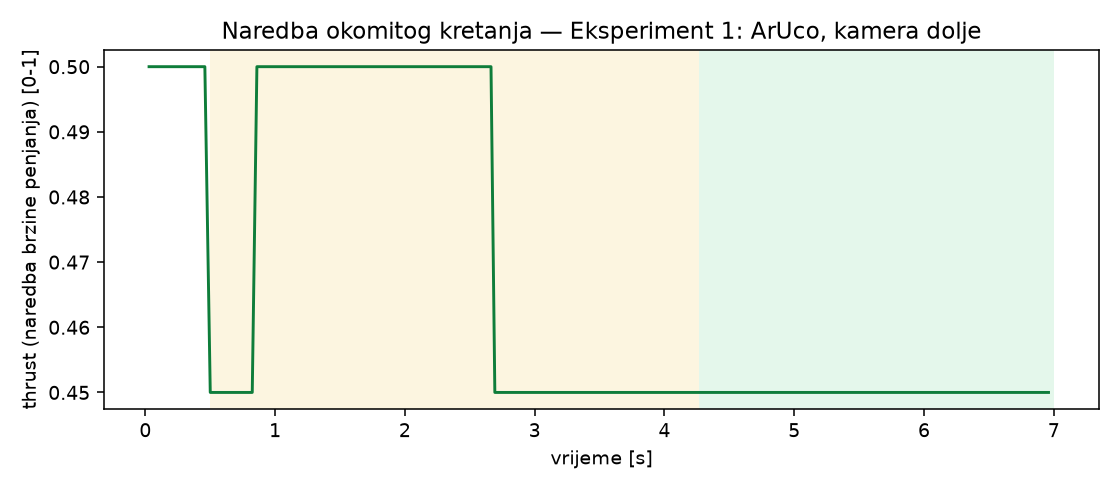
\includegraphics[width=0.85\textwidth]{images/rezultati/exp1_thrust.png}
  \caption{Naredba okomitog kretanja tijekom prvog eksperimenta. Vrijednost 0.5 odgovara mirovanju, niža vrijednost spuštanju.}
  \label{fig:exp1-thrust}
\end{figure}

\subsection{Eksperiment 2: praćenje ArUco oznake (kamera prema gore)}
\label{subsec:rez-eksperiment2}

Nakon preslikavanja osi opisanog u Odjeljku~\ref{subsec:preslikavanje-osi}, letjelica je uspješno poravnala kameru okrenutu prema gore s ArUco oznakom te dosegnula stanje \texttt{ALIGNED}, potvrđujući da preslikavanje osi ispravno funkcionira nakon rotacije kamere za 180 stupnjeva. Nakon ulaska u stanje \texttt{ALIGNED}, pikselna pogreška u ovom konkretnom zapisu nastavlja rasti (Slika~\ref{fig:exp2-error}) sve do povratka u stanje \texttt{ALIGN}, na razini histereznog praga. Ovo ponašanje razmatra se u Odjeljku~\ref{subsec:rasprava-uzdignuti-cilj}. Uz ovu konfiguraciju kamere i istu ArUco detekciju, u zasebnom pokušaju snimljenom na videu letjelica je uspješno izvela i cijeli manevar prijanjanja.

\begin{figure}[h]
  \centering
  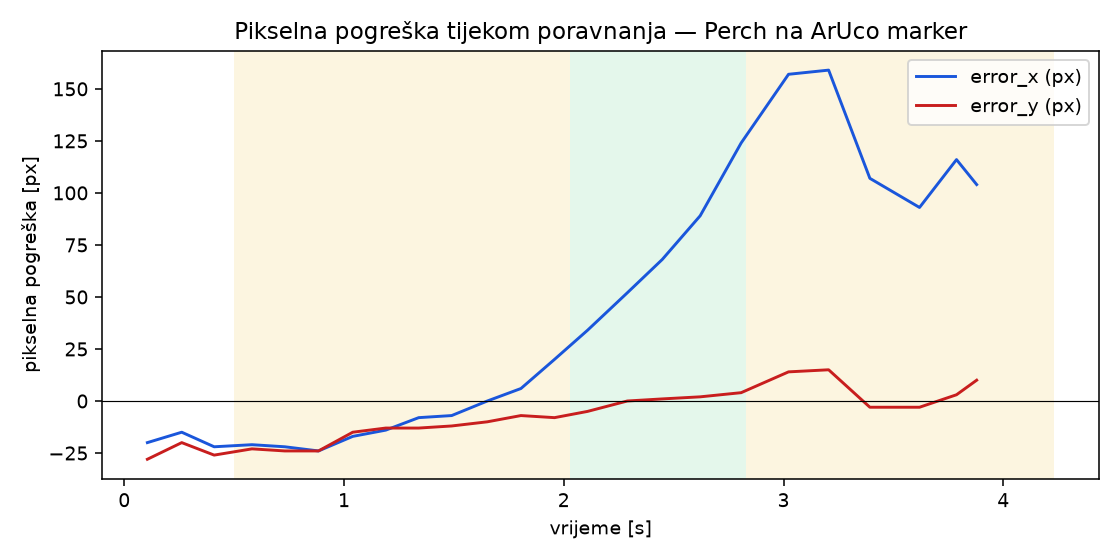
\includegraphics[width=0.85\textwidth]{images/rezultati/exp2_error.png}
  \caption{Pikselna pogreška tijekom drugog eksperimenta. Zeleno osjenčano područje označava stanje \texttt{ALIGNED}.}
  \label{fig:exp2-error}
\end{figure}

\subsection{Eksperiment 3: prijanjanje na granu}
\label{subsec:rez-eksperiment3}

Treći eksperiment rezultirao je uspješnim prijanjanjem na golu granu, bez oznake, korištenjem cjevovoda za detekciju opisanog u poglavlju~\ref{ch:percepcija}. Snimka pokušaja dostupna je kao video prilog radu.

Za uspješni pokušaj, pikselna pogreška (Slika~\ref{fig:exp3-error}) opada iz početne vrijednosti od približno $(-110, -80)$ piksela do nule unutar otprilike 2.7 sekunde, nakon čega slijedi nagli porast pogreške u posljednjoj sekundi prije fizičkog kontakta s granom. Taj porast posljedica je gubitka udaljenosti detekcije od zadanog cilja kako se grana, s približavanjem letjelice, širi preko sve većeg dijela slike i izlazi iz vidnog polja kamere, geometrijski neizbježno u završnoj fazi prijanjanja s kamerom okrenutom prema gore. Letjelica pritom ostaje u stanju \texttt{ALIGN} kroz čitav manevar, sve do naoružavanja isključenog na samom kraju zapisa, nakon fizičkog kontakta s granom. Putanja ciljne točke u slici (Slika~\ref{fig:exp3-target}) potvrđuje tumačenje porasta pogreške: točka se pomiče dijagonalno od gornjeg lijevog dijela slike prema donjem desnom rubu, u skladu sa smjerom u kojem je grana pozicionirana u odnosu na početni položaj letjelice.

Naređeni i stvarni nagib letjelice (Slika~\ref{fig:exp3-rollpitch}) usko prate jedan drugoga do posljednje sekunde prije kontakta, kada dolazi do naglog prekida poravnanja vidljivog u oba grafa kao posljedica gubitka detekcije uslijed kontakta i mehaničkog trzaja pri hvatanju.

\begin{figure}[h]
  \centering
  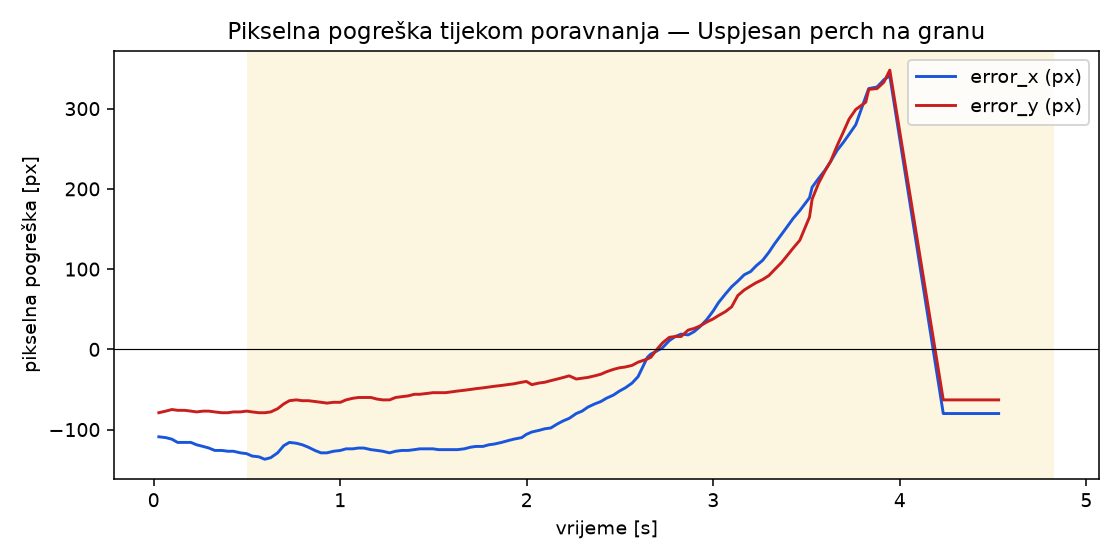
\includegraphics[width=0.85\textwidth]{images/rezultati/exp3_error.png}
  \caption{Pikselna pogreška tijekom uspješnog prijanjanja na granu.}
  \label{fig:exp3-error}
\end{figure}

\begin{figure}[h]
  \centering
  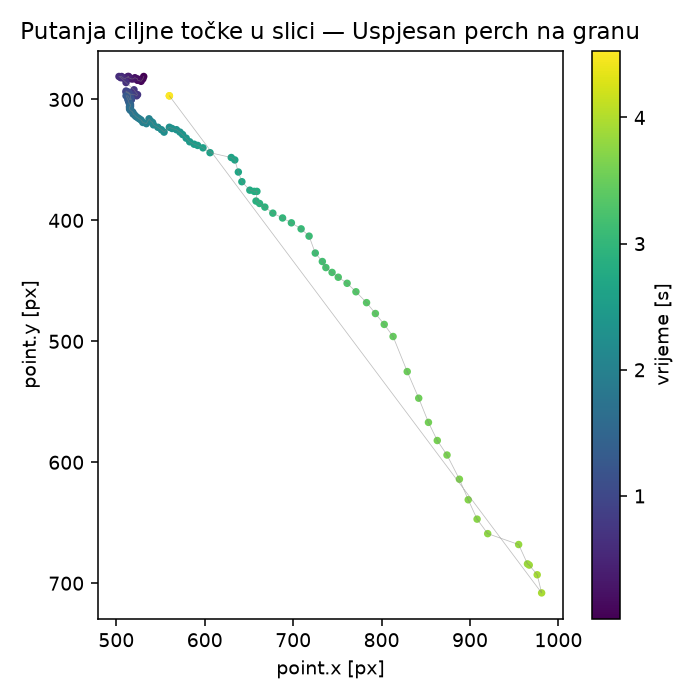
\includegraphics[width=0.6\textwidth]{images/rezultati/exp3_target_traj.png}
  \caption{Putanja ciljne točke u slikovnoj ravnini tijekom uspješnog prijanjanja na granu, obojena prema vremenu.}
  \label{fig:exp3-target}
\end{figure}

\begin{figure}[h]
  \centering
  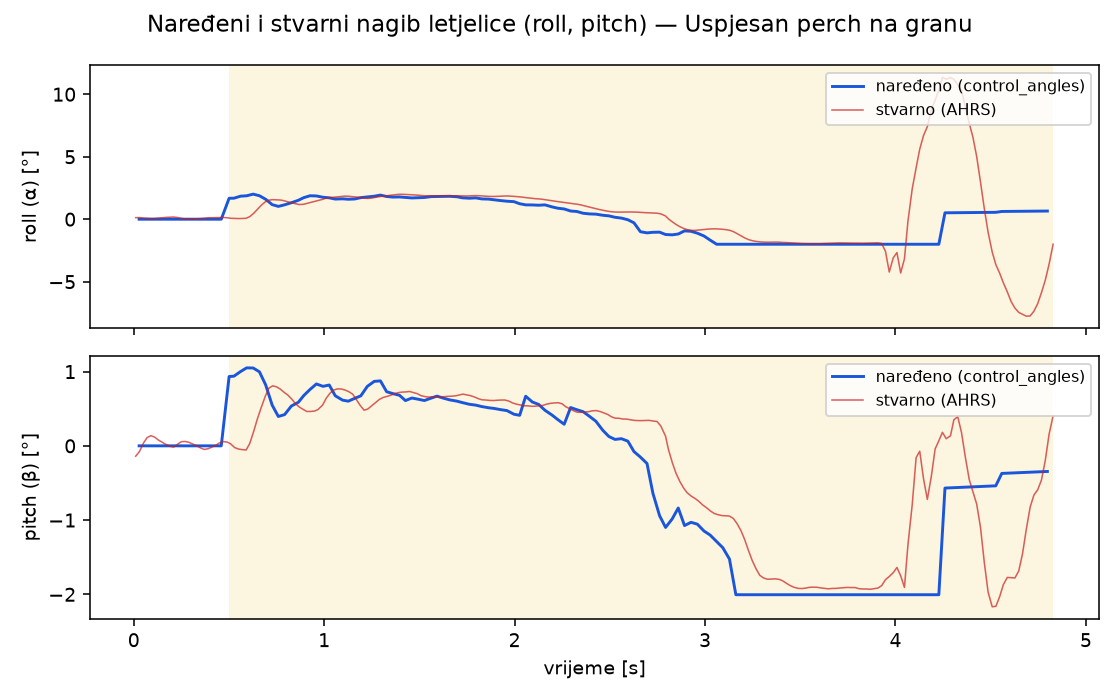
\includegraphics[width=0.85\textwidth]{images/rezultati/exp3_rollpitch.png}
  \caption{Naređeni i stvarni nagib letjelice (roll, pitch) tijekom uspješnog prijanjanja na granu.}
  \label{fig:exp3-rollpitch}
\end{figure}

\begin{figure}[h]
  \centering
  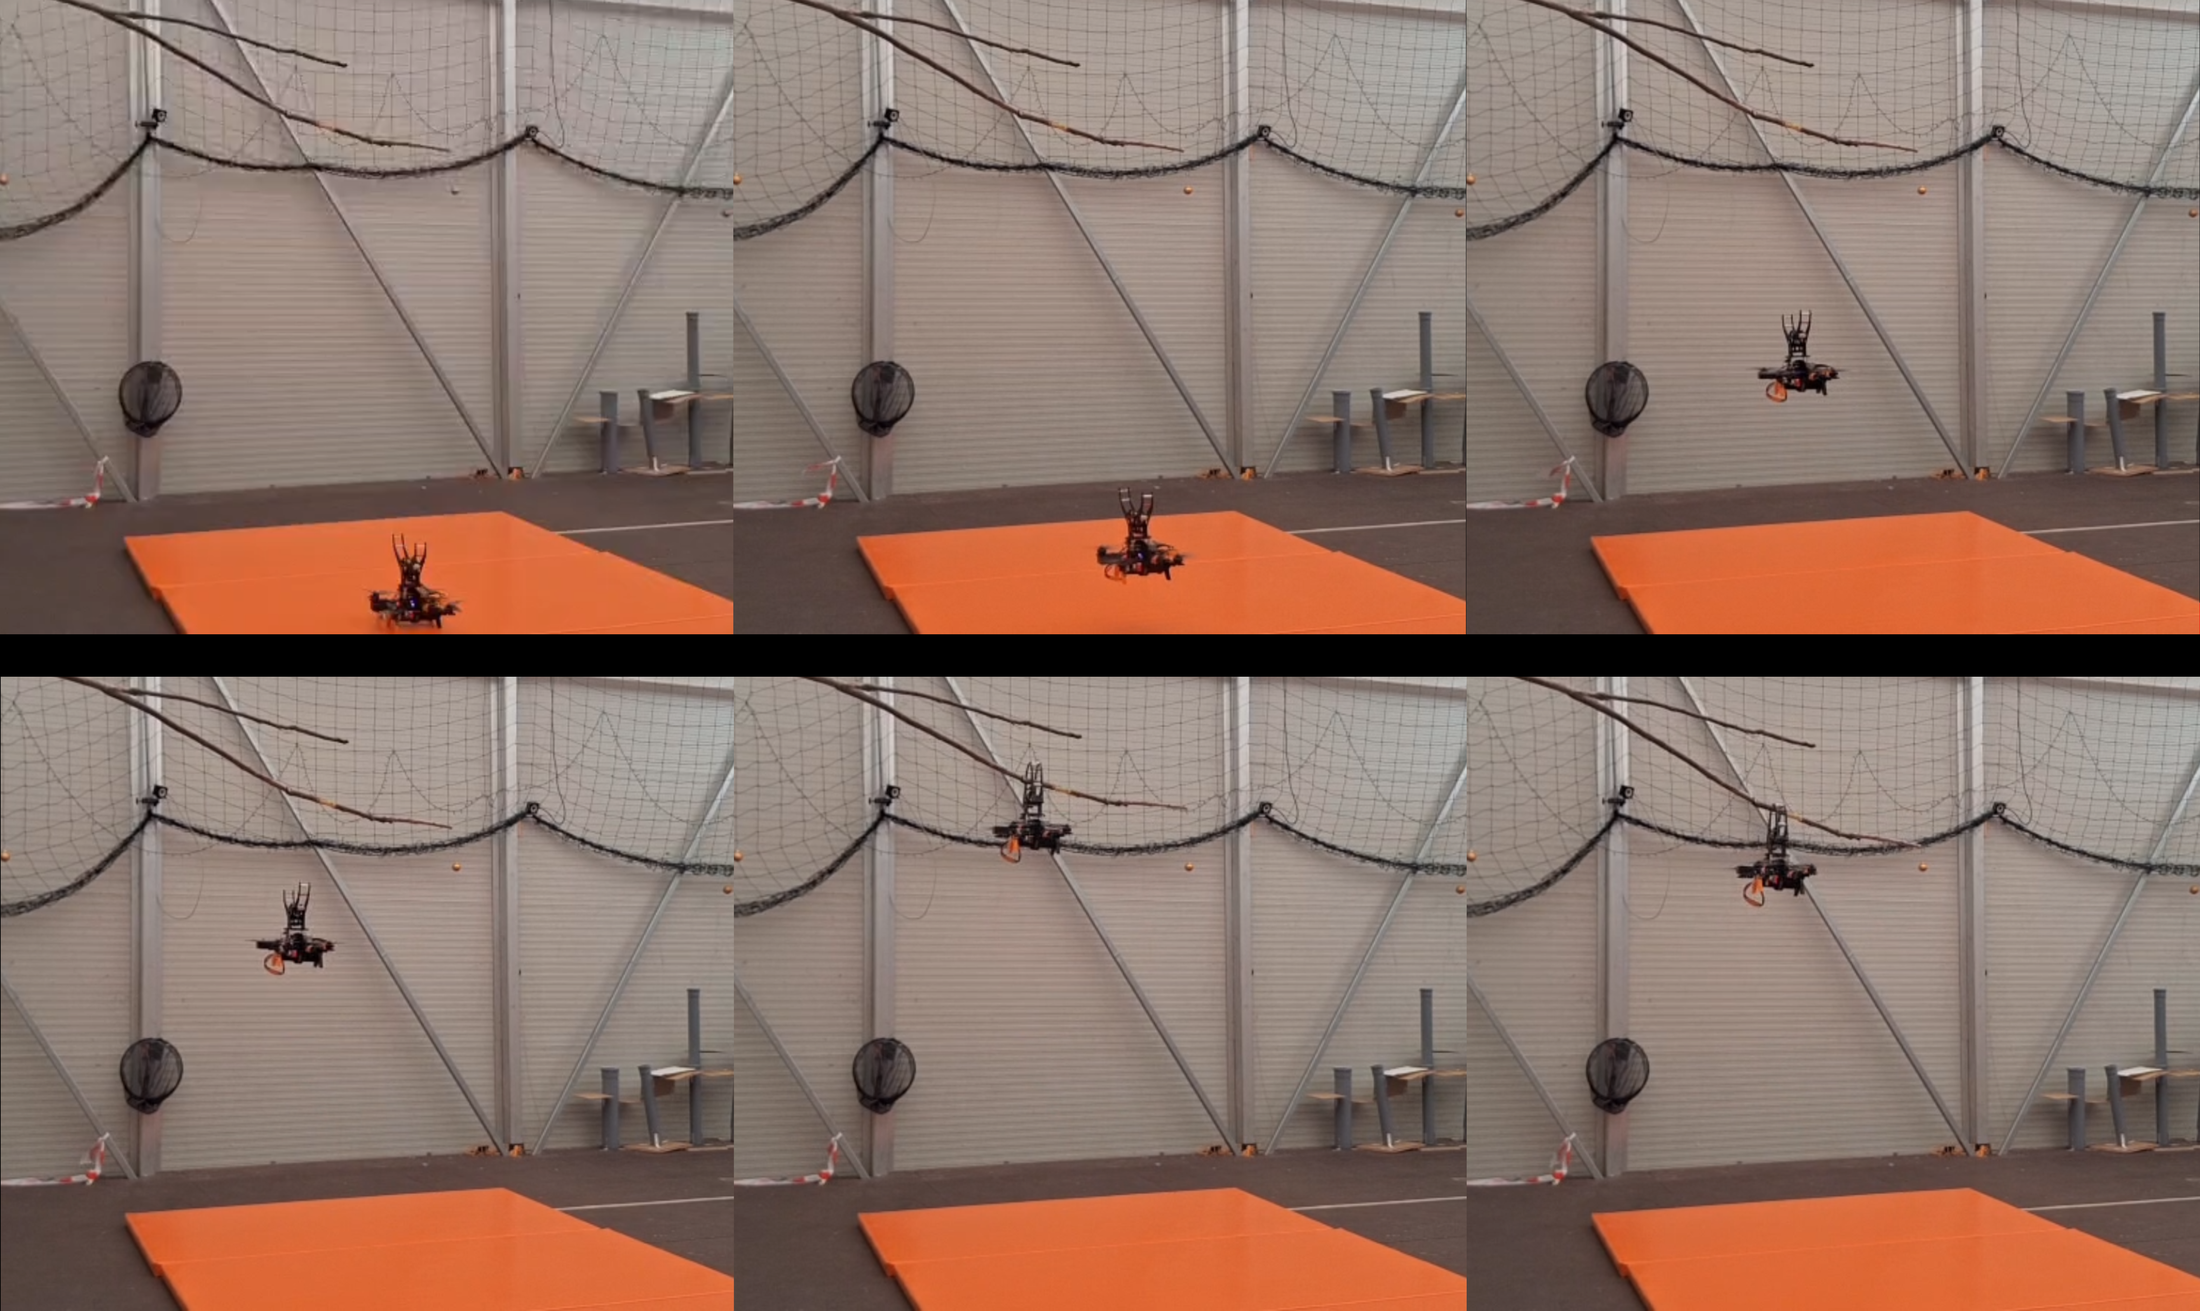
\includegraphics[width=1.0\textwidth]{images/rezultati/exp3_timeline.png}
  \caption{Vremenski slijed uspješnog prijanjanja na granu: uzlijetanje, penjanje, prilazak i hvatanje grane.}
  \label{fig:exp3-success-frame}
\end{figure}

\section{Rasprava}
\label{sec:rasprava}

\subsection{Ostvarenje ciljeva rada}
\label{subsec:rasprava-ciljevi}

Rezultati eksperimenata potvrđuju sva četiri cilja postavljena u Odjeljku~\ref{sec:ciljevi}. Cjevovod za detekciju grane i praćenje točke prijanjanja radi bez ugrađene pretpostavke o orijentaciji kamere, budući da izlaz cjevovoda ostaje jednak pikselnom položaju bez obzira gleda li kamera prema dolje ili prema gore, dok se sva prilagodba geometriji odvija isključivo u preslikavanju osi na upravljačkoj strani (Odjeljak~\ref{subsec:preslikavanje-osi}). Upravljanje letjelicom paketom \texttt{ibvs\_perching} ostvareno je bez vanjske lokalizacije, oslanjajući se isključivo na AHRS procjenu orijentacije i izravno slanje naredbi preko sučelja \texttt{mavros/setpoint\_raw/attitude}, potvrđeno u sva tri eksperimenta. Preslikavanje osi za kameru okrenutu prema gore implementirano je i eksperimentalno potvrđeno drugim i trećim eksperimentom, koji pokazuju da letjelica ispravno poravnava bočni položaj s ciljem iznad sebe. Naposljetku, eksperimentalna provjera provedena je kroz tri opisana koraka rastuće složenosti, pri čemu je treći korak rezultirao uspješnim prijanjanjem na granu bez ijedne oznake ili vanjskog referentnog sustava.

\subsection{Ponašanje nakon dosezanja stanja poravnano}
\label{subsec:rasprava-uzdignuti-cilj}

U drugom eksperimentu (Odjeljak~\ref{subsec:rez-eksperiment2}) pogreška nastavlja rasti i nakon ulaska u stanje \texttt{ALIGNED}, sve do napuštanja tog stanja na histereznom pragu. Ovo je izravna posljedica dizajna praga za spuštanje/penjanje opisanog u Odjeljku~\ref{subsec:prijanjanje}: budući da je taj prag postavljen jednako širokim kao i prag za ulazak u stanje \texttt{ALIGNED}, sustav dopušta rub tolerancije u kojem je letjelica još uvijek unutar dozvoljenog raspona za okomito kretanje, ali izvan raspona koji regulator uspijeva stabilno održavati bez daljnjeg poremećaja. Kod treće provjere, s cjevovodom za detekciju grane, ovo se ponašanje ne očituje na isti način jer manevar prijanjanja završava fizičkim kontaktom s granom prije nego što bi do takvog odstupanja moglo doći.

\subsection{Vezanost pomaka slike i nagiba letjelice}
\label{subsec:rasprava-coupling}

Grafovi pikselne pogreške u sva tri eksperimenta povremeno pokazuju kratkotrajne skokove pogreške usred inače glatkog pada prema nuli. Ovi skokovi nisu posljedica šuma u detekciji, nego izravne fizičke vezanosti (\emph{coupling}) između nagiba letjelice i pomaka slike: kamera je kruto pričvršćena na letjelicu, pa svaki nagib koji regulator naredi radi smanjenja pogreške istovremeno zakreće i sam vidokrug kamere. Taj zakret pomiče cilj u slici u smjeru suprotnom od očekivanog trenutak prije nego što stvarno translacijsko gibanje letjelice počne smanjivati pogrešku, što se u grafu očituje kao kratak, mali porast pogreške upravo u trenutku kada regulator poveća naredbu nagiba. Ova je pojava svojstvena samoj geometriji sustava (kamera kruto vezana za tijelo letjelice bez vlastite stabilizacije nagiba) i ne predstavlja kvar ili nestabilnost regulatora.

\subsection{Održavanje visine pri naredbi mirovanja}
\label{subsec:rasprava-barometar}

Vrijednost naredbe okomitog kretanja 0.5 protumačena je kao naredba mirovanja, odnosno nulte brzine penjanja (Odjeljak~\ref{subsec:prijanjanje}). U idealnim uvjetima to bi značilo da letjelica pri toj naredbi zadržava potpuno nepromijenjenu visinu. U stvarnosti, procjena visine unutar ArduPilota oslanja se na barometarsko mjerenje tlaka, na koje utječe strujanje zraka koje stvaraju vlastiti propeleri letjelice te ograničena preciznost samog barometarskog senzora. Zbog toga naredba mirovanja u praksi ne drži letjelicu na potpuno istoj visini, nego letjelica postupno odstupa dok ArduPilotov regulator visine unutar GUIDED načina rada tu promjenu ne prepozna kao dovoljno značajnu da ju počne aktivno korigirati. Ova nesavršenost održavanja visine dio je razloga za oscilacije vidljive na grafovima naredbe okomitog kretanja, uz vezanost opisanu u Odjeljku~\ref{subsec:rasprava-coupling}.

\subsection{Ograničenje okidanja prijanjanja bez izravnog mjerenja udaljenosti}
\label{subsec:rasprava-okidanje}

Sustav namjerno ne koristi senzor udaljenosti niti bilo kakav diskretni signal za okidanje trenutka prijanjanja (Odjeljak~\ref{subsec:prijanjanje}), nego se penjanje odvija kontinuirano dok je letjelica bočno poravnata, sve dok mehanizam za prijanjanje fizički ne dosegne granu. Ovakav pristup izbjegava ovisnost o dodatnom senzoru, ali prenosi odgovornost za uspješnost hvatanja isključivo na točnost bočnog poravnanja i geometrijski razmak između kamere i hvataljke (Odjeljak~\ref{subsec:test3-postav}). Posljedica je da sustav nema način unaprijed prepoznati da hvatanje neće uspjeti: ako letjelica u trenutku fizičkog kontakta nije dovoljno točno poravnata, manevar se ne zaustavlja niti ponavlja sam od sebe, nego zahtijeva da sigurnosni pilot prekine pokušaj.

\subsection{Utjecaj skupa podataka za treniranje na novu konfiguraciju kamere}
\label{subsec:rasprava-dataset}

Skup podataka za treniranje modela detekcije (Odjeljak~\ref{sec:treniranje-modela}) sniman je pretežno iz bočne perspektive, u skladu s izvornim scenarijem prilaska grani. U scenariju ovog rada, kamera gleda prema gore i grana se u posljednjoj fazi prijanjanja vidi pod znatno oštrijim kutom te bliže rubu ili izvan kadra nego što je slučaj u velikom dijelu skupa za treniranje. Uspješno prijanjanje u trećem eksperimentu pokazuje da model unatoč tome generalizira dovoljno dobro za ovu primjenu, no rastuća pogreška u posljednjoj sekundi prije kontakta (Odjeljak~\ref{subsec:rez-eksperiment3}) dijelom proizlazi i iz ove promjene perspektive, budući da grana pod oštrim kutom zauzima drugačiji oblik u slici nego u većini primjera korištenih za treniranje.



\chapter*{Zahvale}
Zahvaljujem prof.\ dr.\ sc.\ Matku Orsagu i svim članovima LARICS laboratorija na podršci, savjetima i pomoći tijekom izrade ovog rada.

Posebno zahvaljujem Jakobu Domišloviću, mag.\ ing., dr.\ sc.\ Antunu Ivanoviću, Luki Greblu, mag.\ ing., i dr.\ sc.\ Jurici Goričancu na svim savjetima, pomoći pri izvođenju eksperimenata i vremenu koje su uložili tijekom izrade ovog rada.


\printbibliography[heading=bibintoc,title={Popis literature}]

% ============================================================
% SAZETAK / SUMMARY (Prilog 2, tocka 7, podtocke i, j)
% ============================================================
\chapter*{Sažetak}
\noindent\textbf{\imeprezime}

\noindent\textbf{\naslovrada}

\bigskip

\noindent Ovaj rad opisuje prilagodbu upravljačkog sloja bespilotne letjelice za autonomno prijanjanje, namijenjenu scenariju u kojem letjelica polazi već pozicionirana ispod cilja, s kamerom okrenutom prema gore, bez oslanjanja na sustav vanjske lokalizacije i bez korištenja senzora udaljenosti za okidanje manevra prijanjanja. Ciljnu točku u slikovnoj ravnini osigurava percepcijski cjevovod, dok letjelicom izravno upravlja paket \texttt{ibvs\_perching}, slanjem ciljne orijentacije i naredbe brzine penjanja preko MAVROS-a. Rad opisuje potrebno preslikavanje osi između izlaza percepcije i naredbi letjelici u ovoj geometriji te eksperimentalnu provjeru sustava kroz tri koraka rastuće složenosti, od izvorne konfiguracije upravljačkog sloja do potpunog sustava s cjevovodom za detekciju grane. Rezultati potvrđuju da predloženi pristup uspješno ostvaruje prijanjanje bez oznake, oslanjajući se isključivo na pikselnu poziciju cilja i AHRS procjenu orijentacije letjelice.

\bigskip

\noindent\textbf{Ključne riječi:} bespilotna letjelica, prijanjanje, vizualno navođenje temeljeno na slici, autonomno upravljanje, letjelica bez vanjske lokalizacije


\selectlanguage{english}
\chapter*{Summary}
\noindent\textbf{\imeprezime}

\noindent\textbf{\naslovradaEN}

\bigskip

\noindent This paper describes an adaptation of a UAV flight control layer for autonomous perching, for a scenario in which the UAV starts already positioned beneath the target, with the camera facing upward, without relying on external localization and without using a distance sensor to trigger the perching maneuver. The target point in the image plane is provided by a perception pipeline, while the UAV is commanded directly through the \texttt{ibvs\_perching} package, by sending a target orientation and a climb-rate command via MAVROS. The paper describes the axis mapping required between the perception output and the UAV commands in this geometry, and the experimental validation of the system through three steps of increasing complexity, from the control layer's original configuration to the complete system with the branch-detection pipeline. The results confirm that the proposed approach successfully achieves markerless perching, relying solely on the pixel position of the target and the UAV's AHRS orientation estimate.

\bigskip

\noindent\textbf{Key words:} unmanned aerial vehicle, perching, image-based visual servoing, autonomous control, UAV without external localization

\selectlanguage{croatian}

\end{document}
